\documentclass[12pt,openright,twoside]{report}
\usepackage[a4paper,top=25mm,bottom=25mm,right=25mm,left=25mm,bindingoffset=6mm]{geometry}
\usepackage[utf8]{inputenc}
\usepackage[swedish,british]{babel}
\usepackage{amsmath}
\usepackage{graphicx}
\usepackage[dvipsnames]{xcolor}
\usepackage{pict2e}
\usepackage{tabu}
\usepackage{booktabs}
%\usepackage{bookmark,hyperref}
\usepackage[hypertexnames=true]{hyperref}
%\usepackage{hyperref}
\usepackage{gensymb}
\usepackage{wrapfig}
\usepackage{multirow}
\usepackage[nottoc]{tocbibind}

\usepackage{xcolor}
\usepackage{colortbl}
%\usepackage[table]{xcolor}
%\usepackage{tabularray}
\usepackage{watermark}
\usepackage{wallpaper}
\usepackage{eurosym}
\usepackage[toc,title,page]{appendix}
\usepackage{courier}
\usepackage{listings} 
\usepackage{enumitem}
\usepackage{url}
\usepackage{soul}
\usepackage{comment}
\usepackage{parskip}
\usepackage{etoolbox}
\usepackage{float}
\usepackage[T1]{fontenc}
%\usepackage{fontspec}
\graphicspath{{figuren/}}
\usepackage{tikz}
\usetikzlibrary{shapes.geometric, arrows, positioning, fit}


\definecolor{mygray}{gray}{0.85}

\newcommand{\ctext}[3][RGB]{%
	\begingroup
	\definecolor{hlcolor}{#1}{#2}\sethlcolor{hlcolor}%
	\hl{#3}%
	\endgroup
}

\newcommand{\ardIDE}{Arduino IDE 2.3.3}

\newcommand{\specialcell}[2][c]{%
	\begin{tabular}[#1]{@{}c@{}}#2\end{tabular}}

\newcommand*{\img}[1]{%
	\raisebox{-.3\baselineskip}{%
		\includegraphics[
		height=\baselineskip,
		width=\baselineskip,
		keepaspectratio,
		]{#1}%
	}%
}


\input{arduinoLanguage.tex}    % adds the arduino language listing


	
%% Define an Arduino style fore use later %%
\lstset{%
	language=Arduino,
	basicstyle=\footnotesize\ttfamily,
	numbers=left,
	numberstyle=\tiny\color{gray},
	stepnumber=1,                           
	numbersep=8pt,
	%	keywordstyle=\bfseries\color{keyword},
	%	stringstyle=\color{blue},
	%	commentstyle=\itshape\color{comment},
	%	morecomment=[l][\color{cppgreen}]{\#},
	morekeywords=[1]{},                  % [1] -> dark green
	morekeywords=[2]{FILE_WRITE},        % [2] -> light blue
	morekeywords=[3]{SD, File},          % [3] -> bold orange
	morekeywords=[4]{open, exists},      % [4] -> orange
	showspaces=false,
	showstringspaces=false,
	showtabs=false,
	frame=lines,
%	frame=shadowbox,
	rulesepcolor=\color{arduinoBlue},
	rulecolor=\color{black},
	tabsize=4,
	captionpos=b,
	breaklines=true,
	breakatwhitespace=false,
	title=\lstname,
	postbreak=\mbox{\textcolor{red}{$\hookrightarrow$}\space},
	upquote=true,
	aboveskip=1ex,
	belowskip=2ex,
	escapeinside={(*}{*)}
}


%Formatering av rubriker
%%%%%%%%%%%%%%%%%%%%%%%%%%%%%%%%%%%%%%%%%%%%%%%%%%%%%%%%%%%%%%%%%%%%%%%%%%%%%%%%%%%%%%%
\usepackage{titlesec, blindtext, color}
\titleformat{\chapter}[hang]{\Huge\bfseries}{\thechapter}{20pt}{}{}
\titlespacing*{\chapter}{0pt}{*0}{*3}
\titlespacing*{\section}{0pt}{*4}{*1}
\titlespacing*{\subsection}{0pt}{*3}{*0}
\titlespacing*{\subsubsection}{0pt}{*4}{*1}

\setcounter{secnumdepth}{2}
\setcounter{tocdepth}{2}
%%%%%%%%%%%%%%%%%%%%%%%%%%%%%%%%%%%%%%%%%%%%%%%%%%%%%%%%%%%%%%%%%%%%%%%%%%%%%%%%%%%%%%%

\usepackage{tocloft} %Control the ToC formatting

\setlength{\parindent}{0pt}
\setlength{\parskip}{1em}

%Formatting of page numbering (Comment to have the number centered)
%%%%%%%%%%%%%%%%%%%%%%%%%%%%%%%%%%%%%%%%%%%%%%%%%%%%%%%%%%%%%%%%%%%%%%%%%%%%%%%%%%%%%%%
\usepackage{fancyhdr}
\pagestyle{fancyplain}%
\fancyhf{} % clear all header and footer fields
\fancyfoot[RO,LE]{\thepage}
\renewcommand{\headrulewidth}{0pt}
%%%%%%%%%%%%%%%%%%%%%%%%%%%%%%%%%%%%%%%%%%%%%%%%%%%%%%%%%%%%%%%%%%%%%%%%%%%%%%%%%%%%%%%


\usepackage[font=footnotesize,format=plain,labelfont=bf,textfont=sl]{caption}
\usepackage[labelformat=simple,font=footnotesize,format=plain,labelfont=bf,textfont=sl]{subcaption}

\hypersetup{
	colorlinks=true,
	linkcolor=blue,
	filecolor=magenta,      
	urlcolor=cyan,
	pdfnewwindow=true, 
}
%opening
 %  \date{\today}
 \date{}
\title{

{\vspace{-4cm}}
	{\hspace{-20pt}\begin{bfseries}\Huge{\color{black}Technical Skills 2 \\Embedded Systems} \end{bfseries}  } \\
	{(practicumhandleiding micro:bit V2)}
\ThisCenterWallPaper{0.8}{figuren/bbcmicrobitV2.png}

%	\vfill	
	{\vspace{18cm}}	
	{\color{white}  
	\raggedleft  \par}
	Versie 1.34

}


\begin{document}

\maketitle

 \tableofcontents

\let\cleardoublepage\clearpage

% tikzpicture.tex

% Define styles for TikZ elements
\tikzset{
	io/.style = {trapezium, trapezium left angle=80, trapezium right angle=100, minimum width=1cm, minimum height=1cm, text centered, draw=black, fill=blue!30},
	process/.style = {rectangle, minimum width=4cm, minimum height=1cm, text centered, draw=black, fill=orange!30},
	andSetup/.style = {rectangle, minimum width=4cm, minimum height=1cm, text centered, draw=black, fill=yellow!30},
	decision/.style={diamond, minimum width=3cm, minimum height=0.7cm, text centered, draw=black, fill=green!30, aspect=1.5   },
	startstop/.style={rectangle, rounded corners, minimum width=3cm, minimum height=1cm, text centered, draw=black, fill=red!30},
	every ->/.style={ultra thick,>=stealth}
}

\newcommand{\eerstefc}{
	
	\begin{tikzpicture}[node distance=0.4cm]
		\node (start) [startstop] {Start};
%		\node (globaal) [process, below =of start] {Initialisatie teller, eindgetal};
		\node (setup) [andSetup, below = of start]{Zet: COL3-pin en ROW3-pin op output };

	   \node (globaal) [process, below =of setup, yshift=-10pt, align=left] {Initialiseer teller 0\\ Initialiseer eindgetal};
	
		\node [draw, text width=4cm, align=center] (input) [io, below =of globaal]{Voer de waarde van het eindgetal in};
		
		\node (Match) [decision, below =of input,text width=4cm, align=center] {
			 (teller $<$ eindgetal)};
		\node (LEDAan) [process, below =of Match] {Led aan};
		\node (wachtA) [process, below =of LEDAan ] {wacht 500ms};
		\node (LEDUit) [process, below =of wachtA] {Led uit};
		\node (wachtU) [process, below =of LEDUit ] {wacht 500ms};        
		\node (tellerPlus) [process, below =of wachtU] {teller++};
		\node (stop) [startstop,below = of tellerPlus] {Einde loop};
		
		\node[
		draw,
		dashed,
		inner sep=12pt,
		inner xsep=	80pt,
		fit={(globaal) (stop)},
		] (fit) {};
		\node[below right, inner sep=2pt] at (fit.north west) {\small{\textbf{Arduino loop}}};
		
		\draw [->,ultra thick] (start) -- (setup); 
		\draw [->,ultra thick] (setup) -- (globaal);
		
		\draw [->,ultra thick] (globaal) -- (input);

		\draw [->,ultra thick] (input) -- (Match);
		
		\draw [->,ultra thick]  (Match) -- node [anchor=west]{ja}(LEDAan);
		
		\draw [->,ultra thick] (tellerPlus.east)  -- ++(1.5,0) |- (Match.east);
		\draw [->,ultra thick]  (Match.west)  -- +(-1.5,0) |- node[pos=0, anchor=south]{nee} (stop);
%		\draw [->,ultra thick] (setup) -- (input);
		\draw [->,ultra thick] (input) -- (Match);
		\draw [->,ultra thick] (Match) -- (LEDAan);
		\draw [->,ultra thick] (LEDAan) -- (wachtA);
		\draw [->,ultra thick] (wachtA) -- (LEDUit);
		\draw [->,ultra thick] (LEDUit) -- (wachtU);
		\draw [->,ultra thick] (wachtU) -- (tellerPlus);
	\end{tikzpicture}

}

\newcommand{\randomfc}{
	\begin{tikzpicture}[node distance=0.4cm]
	    \node (start) [startstop] {Start};
	    \node (globaal) [process, below =of start] {Adafruit\_Microbit\_Matrix display};
    	\node (setup) [andSetup, below = of globaal]{initialiseer: de Seriele poort,
    	display en randomSeed };
    
	%	\node (globaal) [process, below =of start] {Adafruit_Microbit_Matrix display};
	
		\node (random) [process, below =of setup,yshift=-10pt] {genereer een random getal};
		 \node [draw, text width=4cm, align=center, yshift=-0.5cm] (output) [io, below =of random]{Print: "Voer een decimale waarde in."};
    	\node [draw, text width=4cm, align=center, yshift=-0.5cm] (input) [io, below =of output]{Lees de ingevoerde waarde};


    	\node (Omzet) [process, below =of input] {Zet de ingelezen waarde om naar een integer};
      	\node (Verg) [decision, below =of Omzet,text width=4cm, align=center] {
    		(random getal $=$ ingelezen getal)};
 %   	\node (B) [process, below left=1.5cm and 1cm of Verg, draw] {Node B};
    	\node (Fout) [process, below left =2cm and 0.2cm of Verg] {Helaas, probeer het nog een keer};    	
    	\node (Goed) [process, right =4cm of Fout] {Goed gedaan};
    	
    	\node[
    	draw,
    	dashed,
    	inner sep=12pt,
    	inner xsep=	70pt,
    	xshift=55pt,
    	yshift= -5pt,
    	fit={(random) (Fout)},
    	] (fit) {};
    	\node[below right, inner sep=2pt] at (fit.north west) {\small{\textbf{Arduino loop}}};
    	
     	\draw [->,ultra thick] (start) -- (globaal);
    	\draw [->,ultra thick] (globaal) -- (setup);
    	\draw [->,ultra thick] (setup) -- (random);
      	\draw [->,ultra thick] (random) -- (output);
         \draw [->,ultra thick] (output) -- (input);  	
    	\draw [->,ultra thick] (input) -- (Omzet);
        \draw [->,ultra thick] (Omzet) -- (Verg);  	
         \draw [->,ultra thick] (Verg) -| node [anchor=south] {Nee}(Fout);    	
         \draw [->,ultra thick] (Verg) -| node [anchor=south] {Ja}(Goed);   
          	
	\end{tikzpicture}
}

\newcommand{\derdefc}{
	\begin{tikzpicture}[node distance=0.4cm]
		    \node (start3) [startstop] {Start};
		    \node (globaal3) [process, below =of start3] {Adafruit\_Microbit\_Matrix display};
		    \node (setup3) [andSetup, below = of globaal3]{initialiseer: de Seriele poort, 
		    	display en randomSeed };
	\end{tikzpicture}
	}
%\chapter{Inleiding}


In dit practicum maak je kennis met het programmeren van een Embedded System, in dit geval een 
BBC Micro:bit. Het doel is om je een idee te geven waar je bij de differentiatie ‘Network \& Systems Engineering’ mee te maken krijgt. Daar leer je software te schrijven om hardware aan te sturen.

In dit practicum houden we het simpel. We proberen je analytische vaardigheden te testen, te prikkelen en te ontwikkelen. Je bestudeert de gegeven voorbeelden om de eigenschappen van de hardware en software te ontdekken. Dit doe je tijdens het practicum, op deze manier kun je de docent vragen stellen als het niet duidelijk is en zo kan de docent zien of je met de stof bezig bent.  

Beantwoord vragen Specifiek, Meetbaar, Acceptabel,  Realistisch en op Tijd (SMART). 
Kijk niet alleen wat iets doet, maar vooral hoe iets werkt en waarom. HBO is (ook) analyseren!
De voorbeelden zijn geschreven in de taal C (of C++, afgeleid van C). De taal C is de meest gebruikte taal voor embedded systems.

In het tweede semester van NSE wordt kennisgemaakt met object georiënteerd modelleren en programmeren in de programmeertaal C++. In het vierde semester van NSE wordt dieper ingegaan op embedded software ontwerpen en programmeren in de programmeertalen C en C++. 

We vragen je nu alleen om de code te lezen en te analyseren. Als je Java programmeren in Periode 1 met succes hebt afgerond, dan moet dat lukken. 

De programma’s die je moet maken kun je in elkaar zetten door de code uit de voorbeelden op een slimme manier bij elkaar te kopiëren en te plakken. Zo doe je dat op beginners niveau.

Het belangrijkste doel van het practicum is om een ‘smaakje’ te krijgen van NSE. 
Het practicum ondersteunt op een aantal punten de theorie (zie de leerdoelen op Brightspace). 

Er is in principe géén klassikale instructie. Je werkt zelfstandig aan de hand van deze practicum handleiding. Je kunt wel vragen stellen aan een docent of assistent. Je kunt ook vragen stellen over hoe je de Microbit in ‘The Challenge’ gebruikt, maar je moet zelf de software schrijven.

Er zit geen toetsing in het practicum. De toetsing zit deels in de theorietoets en betreft de opdrachten uit de handleiding. Een aantal opdrachten kan via brightspace ingeleverd worden. Aan de hand van de ingeleverde opdrachten komt een aantekening te staan bij de 'The Challenge' en wordt meegewogen bij het advies dat gegeven wordt indien de NSE richting gekozen wordt. Verdere toetsing zit in jullie uitwerking van het Embedded deel van ‘The Challenge’.

In deze handleiding wordt in hoofdstuk \ref{chap:intr} de eerste opdracht besproken met een aantal basis principes van de arduino omgeving.
Tijdens de tweede opdracht in hoofdstuk \ref{sec:invoer} ligt de nadruk op het invoeren van externe gegeven in een embedded systeem.


In de appendix \ref{chap:omgeving}  wordt de practicum omgeving besproken. In appendix \ref{chap:apB} wordt voor een aantal problemen een oplossing gegeven, verder wordt ingegaan op mogelijke toepassingen bij de challenge.

Voor het practicum heb je een \textbf{eigen laptop, een BBC Microbit en Arduino software} nodig 
(zie de materiaallijst; de Microbit Go kit kost ongeveer \euro{}20). 
\chapter{Inleiding}


In dit practicum maak je kennis met het programmeren van een Embedded System, in dit geval een 
BBC Micro:bit. Het doel is om je een idee te geven waar je bij de differentiatie ‘Network \& Systems Engineering’ mee te maken krijgt. Daar leer je software te schrijven om hardware aan te sturen.

In dit practicum houden we het simpel. We proberen je analytische vaardigheden te testen, te prikkelen en te ontwikkelen. Je bestudeert de gegeven voorbeelden om de eigenschappen van de hardware en software te ontdekken. Dit doe je tijdens het practicum, op deze manier kun je de docent vragen stellen als het niet duidelijk is en zo kan de docent zien of je met de stof bezig bent.  

Beantwoord vragen Specifiek, Meetbaar, Acceptabel,  Realistisch en op Tijd (SMART). 
Kijk niet alleen wat iets doet, maar vooral hoe iets werkt en waarom. HBO is (ook) analyseren!
De voorbeelden zijn geschreven in de taal C (of C++, afgeleid van C). De taal C is de meest gebruikte taal voor embedded systems.

In het tweede semester van NSE wordt kennisgemaakt met object georiënteerd modelleren en programmeren in de programmeertaal C++. In het vierde semester van NSE wordt dieper ingegaan op embedded software ontwerpen en programmeren in de programmeertalen C en C++. 

We vragen je nu alleen om de code te lezen en te analyseren. Als je Java programmeren in Periode 1 met succes hebt afgerond, dan moet dat lukken. 

De programma’s die je moet maken kun je in elkaar zetten door de code uit de voorbeelden op een slimme manier bij elkaar te kopiëren en te plakken. Zo doe je dat op beginners niveau.

Het belangrijkste doel van het practicum is om een ‘smaakje’ te krijgen van NSE. 
Het practicum ondersteunt op een aantal punten de theorie (zie de leerdoelen op Brightspace). 

Er is in principe géén klassikale instructie. Je werkt zelfstandig aan de hand van deze practicum handleiding. Je kunt wel vragen stellen aan een docent of assistent. Je kunt ook vragen stellen over hoe je de Microbit in ‘The Challenge’ gebruikt, maar je moet zelf de software schrijven.

Er zit geen toetsing in het practicum. De toetsing zit deels in de theorietoets en betreft de opdrachten uit de handleiding. Een aantal opdrachten kan via brightspace ingeleverd worden. Aan de hand van de ingeleverde opdrachten komt een aantekening te staan bij de 'The Challenge' en wordt meegewogen bij het advies dat gegeven wordt indien de NSE richting gekozen wordt. Verdere toetsing zit in jullie uitwerking van het Embedded deel van ‘The Challenge’.

In deze handleiding wordt in hoofdstuk \ref{chap:intr} de eerste opdracht besproken met een aantal basis principes van de arduino omgeving.
Tijdens de tweede opdracht in hoofdstuk \ref{sec:invoer} ligt de nadruk op het invoeren van externe gegeven in een embedded systeem.


In de appendix \ref{chap:omgeving}  wordt de practicum omgeving besproken. In appendix \ref{chap:apB} wordt voor een aantal problemen een oplossing gegeven, verder wordt ingegaan op mogelijke toepassingen bij de challenge.

Voor het practicum heb je een \textbf{eigen laptop, een BBC Microbit en Arduino software} nodig 
(zie de materiaallijst; de Microbit Go kit kost ongeveer \euro{}20). 
%\chapter{Opdracht 1\\  \small (Introductie in de Arduino omgeving (week 10 en 11)).}
\label{chap:intr}

Hierbij wordt er van uitgegaan dat:
\begin{enumerate}[label=\alph*)]
	\item Een \hyperref[sec:insArd]{ werkende \ardIDE ~omgeving} aanwezig is.
	\item De \hyperref[sec:instArdOmg] {\ardIDE ~omgeving geschikt is gemaakt voor de microbit}.
	\item De \hyperref[sec:insAdafruit]{ adafruit library} geïnstalleerd is.
\end{enumerate}	 
	 In appendix \ref{chap:omgeving} is te vinden hoe deze te installeren is.\\
	 Verder wordt er vanuit gegaan dat het programmaatje \texttt{\textbf{blink}} zoals in listing \ref{lst:blink} al een keer gerund heeft.

\label{chap:tweeVerv}
Als eerste volgt een korte uitleg aan de hand van het programma \texttt{\textbf{blink}} hoe een Arduino programma in elkaar zit en een korte beschrijving van een paar eigenschappen van de microbit pinnen en de LED-matrix. Verder zijn er een aantal opdrachten. Deze zijn te vinden bij:

\begin{itemize}
	\item Hoofdstuk \ref{sect:mulLED} . Het aanzetten van meerdere LEDs\textbf{ zonder}\\ de \texttt{Adafruit\_Microbit\_Matrix } op bladzijde \pageref{sect:mulLED}.
	\item Het aanzetten van meerdere LEDs met de \texttt{Adafruit\_Microbit\_Matrix}, bladzijde \pageref{blz:opdrmLEDSmatrix}.
	\item Het aantal keren laten knipperen van de LED aan de hand van een ingevoerde waarde, bladzijde \pageref{blad:aantalknipper}. 
	\item Het raden van een binair getal, bladzijde \pageref{blz:bineairGetal}.
	\item Het maken van een looplicht, bladzijde  \pageref{opdr:loppl}.
	\item Het besturen van het looplicht met de accelerometer sensor, bladzijde \pageref{opdr:accSens}.
\end{itemize} 


\section{ Hoe zit een Arduino programma in elkaar?}\label{sec:blink}

We gaan even terug naar het  \href{https://github.com/JohnVi-hhs/embsysP/tree/main/voorbeelden/blink.ino}{  \textbf{blinkdemo}} voorbeeld uit de installatiehandleiding (zie listing \ref{lst:blink}).  Als het goed is heb je deze opgeslagen en kun je deze nu openen.

%\begin{lstlisting}[caption= Het programma blinkdemo.,label={lst:blink}]
	

%\end{lstlisting} 

\begin{lstlisting}[caption= Het programma blinkdemo,label={lst:blink},firstnumber=1]		
const int COL1 = 4;   // Colom #1 control, deze moet 0 zijn
const int LED = 21;   //ROW1 is poort 21.Dit is de linker boven LED.


void setup() {
	
	// omdat de LEDs in een matrix staan moet zowel de plus als de min aangestuurd worden.
	//De stroom loopt immers van + naar -
	pinMode(COL1, OUTPUT); //kolom is de -
	digitalWrite(COL1, LOW);
	pinMode(LED, OUTPUT);  //rij is de +
	
}

void loop() {
	digitalWrite(LED, HIGH);
	delay(500);
	digitalWrite(LED, LOW);
	delay(500);
}
\end{lstlisting}

Arduino noemt een dergelijk programma een schets (of ‘sketch’). 
Hierin zijn twee functieblokken herkenbaar: \texttt{{\textcolor{arduinoBlue}{void}} \textcolor{arduinoGreen}{setup}(){} en  \textcolor{arduinoBlue}{void} \textcolor{arduinoGreen}{loop}(){}}

Wat in het setup blok tussen de accolades \{\} staat, wordt éénmalig tijdens het opstarten uitgevoerd.

Als het setup blok klaar is, wordt het loop blok gestart. De code in het loop blok wordt continue herhaald, in principe duizenden keren per seconde. Het programma eindigt dus nooit, je kunt het niet stoppen!

Deze structuur (een opstartblok en een blok dat herhaald wordt) geldt voor alle type microcontrollers!

Aan het begin van de schets, vóór de \texttt{\textit{ \textcolor{arduinoBlue}{void} \textcolor{arduinoGreen}{setup}()}}, is plek voor het declareren van globale variabelen, deze variabelen kun je overal in het programma gebruiken, zowel in de setup als in de loop.

\colorbox{blue!15}{
	\begin{minipage}{\textwidth}
		Arduino gebruikt \textbf{kleuren} om \textcolor{BurntOrange}{functies} of \textcolor{BlueGreen}{uitdrukkingen} aan te geven. Als je wilt weten wat een dergelijk woord betekent of hoe je het gebruikt, klik dan in de Arduino IDE op het woord en druk 
		\colorbox{mygray}{\textbf{Ctrl + Shift + F}}
		
		Probeer dit uit: Selecteer in Arduino de tekens // en druk \colorbox{mygray}{\textbf{Ctrl + Shift + F}}.

	\end{minipage}
}

De \textcolor{BurntOrange}{oranje gekleurde functies} zijn geen deel van de taal C maar zijn gemaakt door Arduino en zijn gedefinieerd in Arduino libraries die standaard geïnstalleerd zijn. Deze functies maken het leven een stuk makkelijker! Ze vervangen een heleboel moeilijk leesbare C code.

\subsection{Uitleg: Waarom knippert de LED}

Als eerst zal een korte algemene uitleg gegeven worden over het aansturen van een LED, waarna de uitleg volgt in het geval van Listing \ref{lst:blink} besproken wordt.
\paragraph{Het aansturen van een LED:}
Een microcontroller heeft verschillende pinnen die kunnen worden gebruikt als ingangen (input) of uitgangen (output). 
Om een LED aan te sturen wordt vaak de plus-pin van de LED op één van de microcontroller pinnen gezet, de andere pin via een weerstand verbonden met de min. Figuur \ref{fig:exLd} laat zien hoe een externe LED aangesloten is op de micro:kit. De software om de LED  aan te sturen wordt gedaan in Listing \ref{lst:extLd1}.Hierbij is de externe LED aangesloten op poortnummer 8.
\begin{figure}[H]
	\centering
	\begin{center} 	
		\begin{subfigure}[b]{0.43\textwidth}
			\includegraphics[width=0.65\textwidth]{figuren/externeLedCr}
			\caption{Een externe led aangesloten op P08 }
			\label{fig:exLd}
			
		\end{subfigure}
		\begin{subfigure}[b]{0.46\textwidth}
\begin{lstlisting}[caption={Het aansturen van een externe LED.},label={lst:extLd1}]
const int externeLed = 8;
			
void setup() {
	pinMode(externeLed, OUTPUT);  
}
				
void loop() {
  digitalWrite(externeLed,HIGH);
  delay(500);
  digitalWrite(externeLed,LOW);
  delay(500); 
}
\end{lstlisting}
		\end{subfigure}
		\captionsetup{justification=centering}
		\caption{Het aansturen van een externe LED. }
		\label{fig:vbExtld}
	\end{center}	
\end{figure}

De werking van het programma is als volgt.
\begin{enumerate}
	\item In de \textcolor{arduinoGreen}{setup}() wordt dit poortnummer op output gezet,\\  (\textcolor{arduinoOrange}	{pinMode} (externeLed,  \textcolor{arduinoBlue}{OUTPUT})); 
\item In de \textcolor{arduinoGreen}{loop}() wordt:
\begin{enumerate}
	\item Een spanning gezet op poort 8 (\textcolor{arduinoOrange}{digitalWrite}(externeLed, \textcolor{arduinoBlue}{HIGH});) waardoor een elektrische stroom door de LED gaat lopen en deze licht gaat geven. 
	\item Hierna wordt een halve seconde gewacht.
	\item Daarna wordt op poort 8,  0 Volt gezet (\textcolor{arduinoOrange}{digitalWrite}(externeLed, \textcolor{arduinoBlue}{LOW});) en gaat de LED uit (er loopt geen elektrische stroom meer door de LED).
		\item Hierna wordt een halve seconde gewacht.
\end{enumerate} 
\end{enumerate}
 
\subsection{Werken met de LED matrix}

Bij het Blink programma in Listing \ref{lst:blink} wordt een LED aangestuurd dat een onderdeel is van de LED-matrix. De aangestuurde LED \textcolor{blue}{D2} is aangesloten op de pinnen \textcolor{green}{4} en \textcolor{green}{21}  aansluitingen van de LED-matrix wordt in figuur \ref{fig:ledmtx2} weergegeven.


\begin{minipage}{\linewidth}
	\begin{wrapfigure}[23]{r}{0.6\textwidth}
		\vspace{-15pt}
		\begin{center}
			\centering
			\captionsetup{justification=centering}
			\includegraphics[width=0.45\textwidth]{figuren/LedMatrixV2Mnr}
		\end{center}
		%	\vspace{-14pt}
		\caption{Aansluitingen van de LED matrix..}
		\label{fig:ledmtx2}
	\end{wrapfigure}
	
~\vspace{2mm}\\
	Om de LED  (\img{figuren/diodeIc.png}) D2 aan te zetten, zou een elektrische stroom moeten lopen van  pin  \textcolor {Green}{21} door LED D2 naar pin \textcolor{Green}{4}.
	Dit kan voor elkaar verkregen worden door als eerst beide pinnen op output te zetten:\\
	\lstinline|	pinMode(4, OUTPUT);|\\ \lstinline|	pinMode(21, OUTPUT);|\\
	Vervolgens wordt pin \textcolor {Green}{4} laag gemaakt:\\
	 \lstinline|digitalWrite(4,LOW);|\\ en pin \textcolor {Green}{21} hoog gemaakt\\ \lstinline|digitalWrite(21,HIGH);|.\\
	 Indien pin \textcolor {Green}{21}  na een tijdje\\ \lstinline|delay(500);| weer laag wordt gemaakt\\ \lstinline|digitalWrite(21,LOW);| zal de LED uitgaan.
\end{minipage}


\subsection{Het aanzetten van meerdere ledjes in de matrix.}\label{sect:mulLED}

\begin{enumerate}
	
\item In het programma \textit{blink} van listing \ref{lst:blink} knippert de LED met een frequentie van 1 Hz ($\frac{1}{2}$ seconde aan en $\frac{1}{2}$ seconde uit).\\
\begin{enumerate}
	\item Wijzig in de schets de eerste \textcolor{BurntOrange}{delay}(500) (regel 17 van Listing \ref{lst:blink}) naar \textcolor{BurntOrange}{delay}(100).
	\item   Klik op \img{figuren/ardIcUpl.png} of druk \colorbox{mygray}{\textbf{Ctrl + U}} om het programma te compileren en naar de Microbit te sturen.
\end{enumerate}

Je ziet nu dat de ‘aan’ tijd langer is.
\item Laat nu ook LED D6 mee knipperen (LED D2 en D6 knipperen).

\item Laat nu de LEDs D2 en D12 knipperen.

\item Laat nu de LEDs D2, D6 en D12.\\ 
\texttt{Verklaar waarom dit niet eenvoudig lukt en D16 gaat meeknipperen.}


%\item Laad nu ook LED D14 mee knipperen. (LED D2, D6, D12 en D14 Knipperen).\\ %\texttt{Verklaar wat er gebeurt}

\end{enumerate}

\section{De matrix programmeren met behulp van de Adafruit library}\label{sec:matrix}

De firma Adafruit heeft voor de micro:bit een library gemaakt waarin de LED matrix een component is, hierbij worden 5 getallen gebruikt die elk een rij voorstelt. Verder zijn er verschillende methode (functies) die gebruikt kunnen kunnen worden.

De belangrijkste methoden van de Adafruit\textunderscore Microbit\textunderscore Matrix bibliotheek zijn:
\begin{itemize}
	\item begin() om de matrix te initialiseren.
	\item clear() om alle LED's uit te zetten.
	\item drawPixel() om specifieke pixels aan of uit te zetten.
	\item writeDisplay() om de wijzigingen zichtbaar te maken.
	\item drawBitmap() om afbeeldingen weer te geven.
	\item print() om tekst op de matrix te tonen.
\end{itemize}

In Listing \ref{lst:ledmtx} wordt een voorbeeld gegeven van het gebruik van de Adafruit\_Microbit\_Matrix component.

\begin{lstlisting}[caption= Een LED matrix demo,label={lst:ledmtx},firstnumber=1]		
#include <Adafruit_Microbit.h>
Adafruit_Microbit_Matrix ledDisplay;  //definieer de led display

uint8_t led_matrix[] =
{ B00001, // bovenste rij met waarde 1.
	B00010,  //tweede rij  met waarde 2.
	B00100,  //derde rij  met waarde 4.
	8,       //vierde rij  met waarde B01000
	0x10,    //onderste rij met waarde B10000  of terwijl 16
};
void setup() {
	ledDisplay.begin(); 
	ledDisplay.drawPixel(2, 3, 1);  // Zet de LED op positie (2, 3) aan.
	delay(2000);  
	ledDisplay.clear();  
	delay(2000);  
	ledDisplay.show(led_matrix);
}
void loop() {
}
\end{lstlisting}

\paragraph{Opdracht: }Download  \href{https://github.com/JohnVi-hhs/embsysP/tree/main/voorbeelden/matrixOpdracht.ino}{ Listing \ref{lst:ledmtx} van GitHub} of kopieer listing \ref{lst:ledmtx} en 
Pas deze zodanig aan, zodat alleen de LEDs D2, D6 en D12 knipperen.\label{blz:opdrmLEDSmatrix}


\section{Het gebruik van de seriële poort.}

Je kunt de seriële poort gebruiken om informatie te verzenden of te ontvangen van je laptop b.v. om te ‘debuggen’, oftewel controleren of je programma doet wat je er van verwacht. In The Challenge kun je het gebruiken om sensordata naar je PC te sturen. In het voorbeeldprogramma van Listing \ref{lst:serial} wordt de waarde van de teller steeds over de seriële lijn verstuurd.

\begin{lstlisting}[caption= Een LED matrix demo,label={lst:serial},firstnumber=1]		
	
void setup() {
	Serial.begin(9600);
	Serial.println("start");
}
int teller=0;

void loop() {
	Serial.println(teller);
	delay(1000);
	teller++;
}
\end{lstlisting}


Open de seriële monitor(Tools$\rightarrow$Serial Monitor) of (druk \colorbox{mygray}{\textbf{Ctrl + Shift + M}}) of klik op \img{figuren/ardIcMo.png}. In de 'Serial Monitor' verschijnt de output van je programma, zoals te zien is in figuur \ref{fig:arser}
\begin{figure}[H]
	\captionsetup{justification=centering}
	\includegraphics[width=0.5 \linewidth]{figuren/serial}
	\centering
	\caption{Instellingen van de seriële monitor.}
	\label{fig:arser}
\end{figure}
De instellingen van de monitor kan gedaan worden in de statusbalk, zoals te zien is in figuur \ref{fig:arser}.
Vaak wordt 9600 Baud (bits per seconde) gebruikt. Dit is gedaan omdat hiermee de data praktisch altijd stabiel verzonden wordt.

Zorg dat de ingestelde snelheid overeen komt met de instelling \textcolor{BurntOrange}{Serial.begin}(9600) in  \textcolor{OliveGreen}{setup}(). 

%Het programma in Listing \ref{lst:serial}  drukt de waarde van de teller af.\\
\newpage
\paragraph{Opdracht Seriële communicatie:} \label{blad:aantalknipper}
Lees via de seriële poort een getal in en laat een LED het aantal keren knipperen zoals het ingelezen getal. Lees hierna opnieuw een getal in, etc...\\
\textit{Tip:}Lees het getal eerst in als een \href{https://docs.arduino.cc/language-reference/en/functions/communication/serial/readString/}{string} en raadpleeg het voorbeeld dat er bij zit. Zet de ingelezen string vervolgens om naar een integer. Informatie hierover kan gevonden worden bij de arduino referece datatype \href{https://www.arduino.cc/reference/tr/language/variables/data-types/stringobject/}{string}.
\begin{figure}[H]
	\captionsetup{justification=centering}
	\centering
	\eerstefc

	\caption{De LED knippert x keer.}
	\label{fig:flowchart1}
\end{figure}
De flowchart van dit programma wordt weergegeven in figuur \ref{fig:flowchart1}

\paragraph{Opdracht Het binaire getal:} \label{blz:bineairGetal}
Bij deze opdracht wordt een random getal tussen de 0 en de 31 gekozen, die vervolgens op de middelste rij van de led-matrix geplaatst wordt. De gebruiker moet binnen 10 seconden raden wat het getal is. De flowchart van het programma wordt in figuur \ref{fig:flowchart2} weergegeven.
\begin{figure}[H]
	\captionsetup{justification=centering}
	\centering
	\randomfc
	
	\caption{Het raden van de binaire waarde.}
	\label{fig:flowchart2}
\end{figure}

\chapter{Opdracht 1\\  \small (Introductie in de Arduino omgeving (week 10 en 11)).}
\label{chap:intr}

Hierbij wordt er van uitgegaan dat:
\begin{enumerate}[label=\alph*)]
	\item Een \hyperref[sec:insArd]{ werkende \ardIDE ~omgeving} aanwezig is.
	\item De \hyperref[sec:instArdOmg] {\ardIDE ~omgeving geschikt is gemaakt voor de microbit}.
	\item De \hyperref[sec:insAdafruit]{ adafruit library} geïnstalleerd is.
\end{enumerate}	 
	 In appendix \ref{chap:omgeving} is te vinden hoe deze te installeren is.\\
	 Verder wordt er vanuit gegaan dat het programmaatje \texttt{\textbf{blink}} zoals in listing \ref{lst:blink} al een keer gerund heeft.

\label{chap:tweeVerv}
Als eerste volgt een korte uitleg aan de hand van het programma \texttt{\textbf{blink}} hoe een Arduino programma in elkaar zit en een korte beschrijving van een paar eigenschappen van de microbit pinnen en de LED-matrix. Verder zijn er een aantal opdrachten. Deze zijn te vinden bij:

\begin{itemize}
	\item Hoofdstuk \ref{sect:mulLED} . Het aanzetten van meerdere LEDs\textbf{ zonder}\\ de \texttt{Adafruit\_Microbit\_Matrix } op bladzijde \pageref{sect:mulLED}.
	\item Het aanzetten van meerdere LEDs met de \texttt{Adafruit\_Microbit\_Matrix}, bladzijde \pageref{blz:opdrmLEDSmatrix}.
	\item Het aantal keren laten knipperen van de LED aan de hand van een ingevoerde waarde, bladzijde \pageref{blad:aantalknipper}. 
	\item Het raden van een binair getal, bladzijde \pageref{blz:bineairGetal}.
	\item Het maken van een looplicht, bladzijde  \pageref{opdr:loppl}.
	\item Het besturen van het looplicht met de accelerometer sensor, bladzijde \pageref{opdr:accSens}.
\end{itemize} 


\section{ Hoe zit een Arduino programma in elkaar?}\label{sec:blink}

We gaan even terug naar het  \href{https://github.com/JohnVi-hhs/embsysP/tree/main/voorbeelden/blink.ino}{  \textbf{blinkdemo}} voorbeeld uit de installatiehandleiding (zie listing \ref{lst:blink}).  Als het goed is heb je deze opgeslagen en kun je deze nu openen.

%\begin{lstlisting}[caption= Het programma blinkdemo.,label={lst:blink}]
	

%\end{lstlisting} 

\begin{lstlisting}[caption= Het programma blinkdemo,label={lst:blink},firstnumber=1]		
const int COL1 = 4;   // Colom #1 control, deze moet 0 zijn
const int LED = 21;   //ROW1 is poort 21.Dit is de linker boven LED.


void setup() {
	
	// omdat de LEDs in een matrix staan moet zowel de plus als de min aangestuurd worden.
	//De stroom loopt immers van + naar -
	pinMode(COL1, OUTPUT); //kolom is de -
	digitalWrite(COL1, LOW);
	pinMode(LED, OUTPUT);  //rij is de +
	
}

void loop() {
	digitalWrite(LED, HIGH);
	delay(500);
	digitalWrite(LED, LOW);
	delay(500);
}
\end{lstlisting}

Arduino noemt een dergelijk programma een schets (of ‘sketch’). 
Hierin zijn twee functieblokken herkenbaar: \texttt{{\textcolor{arduinoBlue}{void}} \textcolor{arduinoGreen}{setup}(){} en  \textcolor{arduinoBlue}{void} \textcolor{arduinoGreen}{loop}(){}}

Wat in het setup blok tussen de accolades \{\} staat, wordt éénmalig tijdens het opstarten uitgevoerd.

Als het setup blok klaar is, wordt het loop blok gestart. De code in het loop blok wordt continue herhaald, in principe duizenden keren per seconde. Het programma eindigt dus nooit, je kunt het niet stoppen!

Deze structuur (een opstartblok en een blok dat herhaald wordt) geldt voor alle type microcontrollers!

Aan het begin van de schets, vóór de \texttt{\textit{ \textcolor{arduinoBlue}{void} \textcolor{arduinoGreen}{setup}()}}, is plek voor het declareren van globale variabelen, deze variabelen kun je overal in het programma gebruiken, zowel in de setup als in de loop.

\colorbox{blue!15}{
	\begin{minipage}{\textwidth}
		Arduino gebruikt \textbf{kleuren} om \textcolor{BurntOrange}{functies} of \textcolor{BlueGreen}{uitdrukkingen} aan te geven. Als je wilt weten wat een dergelijk woord betekent of hoe je het gebruikt, klik dan in de Arduino IDE op het woord en druk 
		\colorbox{mygray}{\textbf{Ctrl + Shift + F}}
		
		Probeer dit uit: Selecteer in Arduino de tekens // en druk \colorbox{mygray}{\textbf{Ctrl + Shift + F}}.

	\end{minipage}
}

De \textcolor{BurntOrange}{oranje gekleurde functies} zijn geen deel van de taal C maar zijn gemaakt door Arduino en zijn gedefinieerd in Arduino libraries die standaard geïnstalleerd zijn. Deze functies maken het leven een stuk makkelijker! Ze vervangen een heleboel moeilijk leesbare C code.

\subsection{Uitleg: Waarom knippert de LED}

Als eerst zal een korte algemene uitleg gegeven worden over het aansturen van een LED, waarna de uitleg volgt in het geval van Listing \ref{lst:blink} besproken wordt.
\paragraph{Het aansturen van een LED:}
Een microcontroller heeft verschillende pinnen die kunnen worden gebruikt als ingangen (input) of uitgangen (output). 
Om een LED aan te sturen wordt vaak de plus-pin van de LED op één van de microcontroller pinnen gezet, de andere pin via een weerstand verbonden met de min. Figuur \ref{fig:exLd} laat zien hoe een externe LED aangesloten is op de micro:kit. De software om de LED  aan te sturen wordt gedaan in Listing \ref{lst:extLd1}.Hierbij is de externe LED aangesloten op poortnummer 8.
\begin{figure}[H]
	\centering
	\begin{center} 	
		\begin{subfigure}[b]{0.43\textwidth}
			\includegraphics[width=0.65\textwidth]{figuren/externeLedCr}
			\caption{Een externe led aangesloten op P08 }
			\label{fig:exLd}
			
		\end{subfigure}
		\begin{subfigure}[b]{0.46\textwidth}
\begin{lstlisting}[caption={Het aansturen van een externe LED.},label={lst:extLd1}]
const int externeLed = 8;
			
void setup() {
	pinMode(externeLed, OUTPUT);  
}
				
void loop() {
  digitalWrite(externeLed,HIGH);
  delay(500);
  digitalWrite(externeLed,LOW);
  delay(500); 
}
\end{lstlisting}
		\end{subfigure}
		\captionsetup{justification=centering}
		\caption{Het aansturen van een externe LED. }
		\label{fig:vbExtld}
	\end{center}	
\end{figure}

De werking van het programma is als volgt.
\begin{enumerate}
	\item In de \textcolor{arduinoGreen}{setup}() wordt dit poortnummer op output gezet,\\  (\textcolor{arduinoOrange}	{pinMode} (externeLed,  \textcolor{arduinoBlue}{OUTPUT})); 
\item In de \textcolor{arduinoGreen}{loop}() wordt:
\begin{enumerate}
	\item Een spanning gezet op poort 8 (\textcolor{arduinoOrange}{digitalWrite}(externeLed, \textcolor{arduinoBlue}{HIGH});) waardoor een elektrische stroom door de LED gaat lopen en deze licht gaat geven. 
	\item Hierna wordt een halve seconde gewacht.
	\item Daarna wordt op poort 8,  0 Volt gezet (\textcolor{arduinoOrange}{digitalWrite}(externeLed, \textcolor{arduinoBlue}{LOW});) en gaat de LED uit (er loopt geen elektrische stroom meer door de LED).
		\item Hierna wordt een halve seconde gewacht.
\end{enumerate} 
\end{enumerate}
 
\subsection{Werken met de LED matrix}

Bij het Blink programma in Listing \ref{lst:blink} wordt een LED aangestuurd dat een onderdeel is van de LED-matrix. De aangestuurde LED \textcolor{blue}{D2} is aangesloten op de pinnen \textcolor{green}{4} en \textcolor{green}{21}  aansluitingen van de LED-matrix wordt in figuur \ref{fig:ledmtx2} weergegeven.


\begin{minipage}{\linewidth}
	\begin{wrapfigure}[23]{r}{0.6\textwidth}
		\vspace{-15pt}
		\begin{center}
			\centering
			\captionsetup{justification=centering}
			\includegraphics[width=0.45\textwidth]{figuren/LedMatrixV2Mnr}
		\end{center}
		%	\vspace{-14pt}
		\caption{Aansluitingen van de LED matrix..}
		\label{fig:ledmtx2}
	\end{wrapfigure}
	
~\vspace{2mm}\\
	Om de LED  (\img{figuren/diodeIc.png}) D2 aan te zetten, zou een elektrische stroom moeten lopen van  pin  \textcolor {Green}{21} door LED D2 naar pin \textcolor{Green}{4}.
	Dit kan voor elkaar verkregen worden door als eerst beide pinnen op output te zetten:\\
	\lstinline|	pinMode(4, OUTPUT);|\\ \lstinline|	pinMode(21, OUTPUT);|\\
	Vervolgens wordt pin \textcolor {Green}{4} laag gemaakt:\\
	 \lstinline|digitalWrite(4,LOW);|\\ en pin \textcolor {Green}{21} hoog gemaakt\\ \lstinline|digitalWrite(21,HIGH);|.\\
	 Indien pin \textcolor {Green}{21}  na een tijdje\\ \lstinline|delay(500);| weer laag wordt gemaakt\\ \lstinline|digitalWrite(21,LOW);| zal de LED uitgaan.
\end{minipage}


\subsection{Het aanzetten van meerdere ledjes in de matrix.}\label{sect:mulLED}

\begin{enumerate}
	
\item In het programma \textit{blink} van listing \ref{lst:blink} knippert de LED met een frequentie van 1 Hz ($\frac{1}{2}$ seconde aan en $\frac{1}{2}$ seconde uit).\\
\begin{enumerate}
	\item Wijzig in de schets de eerste \textcolor{BurntOrange}{delay}(500) (regel 17 van Listing \ref{lst:blink}) naar \textcolor{BurntOrange}{delay}(100).
	\item   Klik op \img{figuren/ardIcUpl.png} of druk \colorbox{mygray}{\textbf{Ctrl + U}} om het programma te compileren en naar de Microbit te sturen.
\end{enumerate}

Je ziet nu dat de ‘aan’ tijd langer is.
\item Laat nu ook LED D6 mee knipperen (LED D2 en D6 knipperen).

\item Laat nu de LEDs D2 en D12 knipperen.

\item Laat nu de LEDs D2, D6 en D12.\\ 
\texttt{Verklaar waarom dit niet eenvoudig lukt en D16 gaat meeknipperen.}


%\item Laad nu ook LED D14 mee knipperen. (LED D2, D6, D12 en D14 Knipperen).\\ %\texttt{Verklaar wat er gebeurt}

\end{enumerate}

\section{De matrix programmeren met behulp van de Adafruit library}\label{sec:matrix}

De firma Adafruit heeft voor de micro:bit een library gemaakt waarin de LED matrix een component is, hierbij worden 5 getallen gebruikt die elk een rij voorstelt. Verder zijn er verschillende methode (functies) die gebruikt kunnen kunnen worden.

De belangrijkste methoden van de Adafruit\textunderscore Microbit\textunderscore Matrix bibliotheek zijn:
\begin{itemize}
	\item begin() om de matrix te initialiseren.
	\item clear() om alle LED's uit te zetten.
	\item drawPixel() om specifieke pixels aan of uit te zetten.
	\item writeDisplay() om de wijzigingen zichtbaar te maken.
	\item drawBitmap() om afbeeldingen weer te geven.
	\item print() om tekst op de matrix te tonen.
\end{itemize}

In Listing \ref{lst:ledmtx} wordt een voorbeeld gegeven van het gebruik van de Adafruit\_Microbit\_Matrix component.

\begin{lstlisting}[caption= Een LED matrix demo,label={lst:ledmtx},firstnumber=1]		
#include <Adafruit_Microbit.h>
Adafruit_Microbit_Matrix ledDisplay;  //definieer de led display

uint8_t led_matrix[] =
{ B00001, // bovenste rij met waarde 1.
	B00010,  //tweede rij  met waarde 2.
	B00100,  //derde rij  met waarde 4.
	8,       //vierde rij  met waarde B01000
	0x10,    //onderste rij met waarde B10000  of terwijl 16
};
void setup() {
	ledDisplay.begin(); 
	ledDisplay.drawPixel(2, 3, 1);  // Zet de LED op positie (2, 3) aan.
	delay(2000);  
	ledDisplay.clear();  
	delay(2000);  
	ledDisplay.show(led_matrix);
}
void loop() {
}
\end{lstlisting}

\paragraph{Opdracht: }Download  \href{https://github.com/JohnVi-hhs/embsysP/tree/main/voorbeelden/matrixOpdracht.ino}{ Listing \ref{lst:ledmtx} van GitHub} of kopieer listing \ref{lst:ledmtx} en 
Pas deze zodanig aan, zodat alleen de LEDs D2, D6 en D12 knipperen.\label{blz:opdrmLEDSmatrix}


\section{Het gebruik van de seriële poort.}

Je kunt de seriële poort gebruiken om informatie te verzenden of te ontvangen van je laptop b.v. om te ‘debuggen’, oftewel controleren of je programma doet wat je er van verwacht. In The Challenge kun je het gebruiken om sensordata naar je PC te sturen. In het voorbeeldprogramma van Listing \ref{lst:serial} wordt de waarde van de teller steeds over de seriële lijn verstuurd.

\begin{lstlisting}[caption= Een LED matrix demo,label={lst:serial},firstnumber=1]		
	
void setup() {
	Serial.begin(9600);
	Serial.println("start");
}
int teller=0;

void loop() {
	Serial.println(teller);
	delay(1000);
	teller++;
}
\end{lstlisting}


Open de seriële monitor(Tools$\rightarrow$Serial Monitor) of (druk \colorbox{mygray}{\textbf{Ctrl + Shift + M}}) of klik op \img{figuren/ardIcMo.png}. In de 'Serial Monitor' verschijnt de output van je programma, zoals te zien is in figuur \ref{fig:arser}
\begin{figure}[H]
	\captionsetup{justification=centering}
	\includegraphics[width=0.5 \linewidth]{figuren/serial}
	\centering
	\caption{Instellingen van de seriële monitor.}
	\label{fig:arser}
\end{figure}
De instellingen van de monitor kan gedaan worden in de statusbalk, zoals te zien is in figuur \ref{fig:arser}.
Vaak wordt 9600 Baud (bits per seconde) gebruikt. Dit is gedaan omdat hiermee de data praktisch altijd stabiel verzonden wordt.

Zorg dat de ingestelde snelheid overeen komt met de instelling \textcolor{BurntOrange}{Serial.begin}(9600) in  \textcolor{OliveGreen}{setup}(). 

%Het programma in Listing \ref{lst:serial}  drukt de waarde van de teller af.\\
\newpage
\paragraph{Opdracht Seriële communicatie:} \label{blad:aantalknipper}
Lees via de seriële poort een getal in en laat een LED het aantal keren knipperen zoals het ingelezen getal. Lees hierna opnieuw een getal in, etc...\\
\textit{Tip:}Lees het getal eerst in als een \href{https://docs.arduino.cc/language-reference/en/functions/communication/serial/readString/}{string} en raadpleeg het voorbeeld dat er bij zit. Zet de ingelezen string vervolgens om naar een integer. Informatie hierover kan gevonden worden bij de arduino referece datatype \href{https://www.arduino.cc/reference/tr/language/variables/data-types/stringobject/}{string}.
\begin{figure}[H]
	\captionsetup{justification=centering}
	\centering
	\eerstefc

	\caption{De LED knippert x keer.}
	\label{fig:flowchart1}
\end{figure}
De flowchart van dit programma wordt weergegeven in figuur \ref{fig:flowchart1}

\paragraph{Opdracht Het binaire getal:} \label{blz:bineairGetal}
Bij deze opdracht wordt een random getal tussen de 0 en de 31 gekozen, die vervolgens op de middelste rij van de led-matrix geplaatst wordt. De gebruiker moet binnen 10 seconden raden wat het getal is. De flowchart van het programma wordt in figuur \ref{fig:flowchart2} weergegeven.
\begin{figure}[H]
	\captionsetup{justification=centering}
	\centering
	\randomfc
	
	\caption{Het raden van de binaire waarde.}
	\label{fig:flowchart2}
\end{figure}


\section{Bitwise operaties.}
\label{chap:biw}

Zoals in hoofdstuk \ref{sec:matrix} staat vermeldt heeft de firma Adafruit voor het matrix display een speciale component gemaakt waardoor het matrix display eenvoudig te programmeren is. Listing \ref{lst:matrixaan} is hier een voorbeeld van.
\begin{lstlisting}[caption={Het aanzetten van een LED},label={lst:matrixaan}]
#include <Adafruit_Microbit.h>
#define LED0 0  //definieer LEDx tot een waarde
#define LED1 1
#define LED2 2
#define LED3 3
#define LED4 4

Adafruit_Microbit_Matrix matrixMbit; //maak een LED matrix aan.
const uint8_t
smile_bmp[] =
{ B00000,
	B01010,
	B00000,
	B10001,
	B01110, };
uint8_t matrixje[] =
{ B00000,
	B00000,
	B00000,
	B00000,
	B00000, };

void setup() {
	Serial.begin(9600);
	Serial.println("Welkom bij embedded!");
	
	matrixMbit.begin();
	matrixMbit.show(smile_bmp);
	delay(2000);
	matrixMbit.show(matrixje);
	delay(2000);  
	//zet rechterLED bovenste rij aan
	matrixje[0]= 1 << LED0; //schuif 1, LED0 plaatsen op naar links.
	matrixMbit.show(matrixje);
	delay(2000);  
	//zet linkerLED bovenste rij aan 
	matrixje[0] = 1 << LED4; //schuif 1, LED4 plaatsen op naar links.
	matrixMbit.show(matrixje);
}
void loop() {
}
\end{lstlisting}
Wat opvalt aan Listing \ref{lst:matrixaan} is dat er een hoop define's staan aan het begin. De bedoeling van deze define's is dat de code eenvoudiger te lezen is.
Indien in de code  \small{\texttt{\textit{1 \textless\textless  ~LED4}}} staat, weet de lezer gelijk dat de $4^{e}$ LED bedoeld wordt. Verder is te zien hoe een LED aangezet kan worden door de betreffende bit in een array van 8 bits data, een 1 te maken. Dit wordt gedaan door een 1 (0b00000001) een aantal plaatsen naar links op te laten schuiven. Zoals te zien is in onderstaand statement:\\
\texttt{\textit{matrixje[0]= 1 \textless\textless  ~LED0;}}\\
Hierbij staat de \texttt{1} voor het aantal plaatsen dat LED0 naar links wordt opgeschoven. LED0 staat gedefinieerd op regel 2 van Listing \ref{lst:matrixaan}
\begin{enumerate}
	\item Installeer \href{https://learn.adafruit.com/use-micro-bit-with-arduino/adafruit-libraries}{de Adafruit Libraries} indien dit nog niet gedaan is.
	\item
	\begin{enumerate}

	\item Open voorbeeldcode matrixSmpl (dit is Listing \ref{lst:matrixaan}). 
	\item Breid het programma zodanig zodat uit, zodat zowel LED0 als LED4 van de 2e rij aangaan. Maak hierbij gebruik van de operatoren '\textless\textless' en '\textbar'(bitwise or). Doe dit zoals in de theorie besproken is.
	
%	\begin{table}[h!]
\setlength\arrayrulewidth{2pt}
		\begin{tabular}{|c|c|c|}
			\hline
%			\colorbox{yellow}{\textbf{A}} &\colorbox{yellow}{\textbf{B} & \colorbox{Yellow}{\textbf{AB}}   \\ \hline
          \rowcolor{yellow}
		    A  & B     & A \textbar~ B       \\ \hline          
		    0  & 0     & 0       \\ \hline
			0      & 1     & 1       \\ \hline
			1     & 0     & 1       \\ \hline
			1    & 1     & 1       \\ \hline
		\end{tabular}\\
De bitwise OR 
%	\end{table}
	
	\item Breid het programma uit zodat 2 seconde nadat beide LEDS uit B aangegaan zijn, de linker boven LED (LED4) weer uitgaat. Maak hierbij gebruik van de operatoren '\textless\textless' ,  '\&' en  ' $\sim$'. Doe dit zoals in de theorie besproken is.
	
	\setlength\arrayrulewidth{2pt}
	\begin{tabular}{|c|c|c|}
		\hline
		%			\colorbox{yellow}{\textbf{A}} &\colorbox{yellow}{\textbf{B} & \colorbox{Yellow}{\textbf{AB}}   \\ \hline
		\rowcolor{yellow}
		A  & B     & A \& B       \\ \hline          
		0  & 0     & 0       \\ \hline
		0      & 1     & 0       \\ \hline
		1     & 0     & 0       \\ \hline
		1    & 1     & 1       \\ \hline
	\end{tabular}\\
	De bitwise AND 
	\item Door met bitwise operaties te werken, kan op een eenvoudige wijze een LED dat aan is, uitgezet worden en een LED dat uit is aangezet worden. Dit kan gedaan worden met de exclusief OR operator, zoals te zien is in onderstaand tabel. 
	Breid het programma uit zodat 2 LEDS van de onderste rij aan en uitgaan door de exclusief OR functie te gebruiken. Maak hierbij onder ander gebruik van de operator \^ ~. Do dit zoals in de theorie besproken is.
	
	\setlength\arrayrulewidth{2pt}
	\begin{tabular}{|c|c|c|}
		\hline
		%			\colorbox{yellow}{\textbf{A}} &\colorbox{yellow}{\textbf{B} & \colorbox{Yellow}{\textbf{AB}}   \\ \hline
		\rowcolor{yellow}
		A  & B     & A \^ ~ B       \\ \hline          
		0  & 0     & 0       \\ \hline
		0      & 1     & 1       \\ \hline
		1     & 0     & 1      \\ \hline
		1    & 1     & 0       \\ \hline
	\end{tabular}\\
	De bitwise XOR 
	
	\item Er kan ook getest worden of een LED aan is met behulp van bitwise operatoren.\\	\textcolor{cyan}{uint8\_t} hulpje= matrixje[0];\\
	\textcolor{OliveGreen}{if}(hulpje ...  .....) \{ \\
\}.

Vul het \textcolor{arduinoGreen}{if} statement in en toon aan dat een LED aan of uit is.
 \end{enumerate}

\item In het volgende voorbeeld gaat steeds een LED van rechts naar links aan.

\begin{lstlisting}[caption={Looplicht van de bovenste rij.},label={lst:matrixaan2}]
#include <Adafruit_Microbit.h>

Adafruit_Microbit_Matrix matrixMbit; //maak een LED matrix aan.

uint8_t matrixje[] =
{ B00000,
	B00000,
	B00000,
	B00000,
	B00000, };

void setup() {
	Serial.begin(9600);
	Serial.println("Welkom bij embedded!");

    matrixMbit.begin();
	matrixMbit.show(matrixje);
	delay(1000);  
}

uint8_t nr=0;
uint8_t hulpje;

void loop() {
	hulpje = 1 << nr; //schuif 1, nr plaatsen op naar links.
	matrixje[0]=hulpje; //De bovenste rij van de matrix krijgt de 
	matrixMbit.show(matrixje);
	delay(1000);
	nr++;
	if (nr == 5) {
	    nr=0;
	}        
}
\end{lstlisting}
Op regel 5 wordt een matrix component aangemaakt. Het tonen van de matrix wordt met de show functie gedaan (regel 16 en en 26).

\begin{enumerate}
	\item Download de  \href{https://github.com/JohnVi-hhs/embsysP/tree/main/voorbeelden/matrixloopl.ino}{voorbeeldcode van GitHub} of van brightspace of kopieer listing \ref{lst:matrixaan} in een nieuwe Arduino schets en voer deze uit.\\
	Probeer de uitvoer te verklaren.

\item Maak een functie \texttt{void \textit{zetLedAan}(unint8\_t rij,uint8\_t kolom);} die de LED op kolom en rij aanzet. Maak hierbij gebruik van de bitwise operator \textbar ~ zoals besproken tijdens de les.
\item Maak een functie \texttt{void \textit{zetLedUit}(unint8\_t rij,uint8\_t kolom);} die de LED op kolom en rij uitzet. Maak hierbij gebruik van de bitwise operatoren \& en $\sim$ zoals besproken tijdens de les.
\item Maak een functie \texttt{bool \textit{isLedAan}(unint8\_t rij,uint8\_t kolom);} die checkt of de LED op kolom en rij aan is. Maak hierbij gebruik van een bitmasker zoals besproken tijdens de les.

	\item Pas listing \ref{lst:matrixaan} met behulp van de bovenstaande functies zodanig aan, zodat:
\begin{enumerate}%[label=\arabic*.]
	\item Nadat de eerste rij geweest is, bij de tweede rij de ledjes \'{e}\'{e}n voor \'{e}\'{e}n  aangaan. 
	\item Na de tweede rij bij de derde rij de ledjes \'{e}\'{e}n voor \'{e}\'{e}n  aan gaan. 
	\item Na de laatste rij bij de eerste rij de ledjes \'{e}\'{e}n voor \'{e}\'{e}n  aan gaan. 
\end{enumerate}

\textbf{Upload het resultaat op brightspace.}
\end{enumerate}\label{opdr:loppl}
\item Maak een looplicht dat gaat over alle 5 de rijen van de matrix zoals figuur \ref{fig:loopl} laat zien.

\begin{figure}[H]
	\captionsetup{justification=centering}
\includegraphics[width=0.6 \linewidth]{figuren/looplicht}
\centering
\caption{De volgorde van het looplicht.}
\label{fig:loopl}
\end{figure}

Begin rechtsboven (bit 0 van de ${0^{e}}$ rij in de matrix) en zet vervolgens steeds de LED links aan. Doe dit tot laatste LED van de rij.
Ga 1 rij naar beneden en zet vervolgens de LED rechts van de rij aan. Doe dit tot en met het $1^{e}$ bit.
Ga 1 rij naar beneden en zet vervolgens de LED links van de rij aan. Doe dit tot en met de laatste LED en ga vervolgens een rij naar beneden.
Doe dit tot en met de laatste rij en begin vervolgens weer op de eerste rij, zoals in het volgende filmpje \href{https://www.youtube.com/shorts/8ZyYWEiXsm0} {
	looplicht}
	te zien is.\\
\textbf{Upload het resultaat op brightspace.}
\end{enumerate}

\paragraph{Challenge opdracht}\label{opdr:accSens}

Op de micro:bit zitten verschillende sensoren. Eén van de sensoren is een \href{https://youtu.be/9WAckt2vrrQ}{accelerometer sensor}.
Het programma in listing \ref{lst:acc} toont de x,y en z waarde van de accelerator sensor.
\begin{enumerate}

	\item Download  listing \ref{lst:acc} van \href{https://github.com/JohnVi-hhs/embsysP/tree/main/voorbeelden/accelerator.ino}{ GitHub} of van brightspace of kopieer listing \ref{lst:acc} in een nieuwe arduino omgeving en voer deze uit.
	\item Pas het programma zodanig aan, zodat de LED in de richting beweegt, waarin micro:kit gehouden wordt.

	\end{enumerate}

\begin{lstlisting}[caption={Looplicht van de bovenste rij.},label={lst:acc}]
#include <LSM303AGR_ACC_Sensor.h>

#define DEV_I2C Wire1   // Wire1 is voor de interne I2C bus 
#define LED ROW1 


// Nodig voor de accelerator 
LSM303AGR_ACC_Sensor Acc(&DEV_I2C);


const int COL1 = 4;   
const int ROW1 = 21;   

void setup() {
	// Led.
	
	pinMode(COL1, OUTPUT);
	digitalWrite(COL1, LOW);
	pinMode(ROW1, OUTPUT);
	
	// Initialisatie van de serieele.
	Serial.begin(9600);
	
	// Initialisate I2C bus (wordt veel gebruikt om sensors).
	DEV_I2C.begin();
	
	// Initialisatie van de accelarator.
	Acc.begin();
	Acc.Enable();
	
	uint8_t a;
	Acc.IO_Read(&a,0x0F,1);
	Serial.print("Ik ben: ");
	Serial.println(a);
}

void loop() {
	// Led blinking.
	digitalWrite(LED, HIGH);
	delay(250);
	digitalWrite(LED, LOW);
	delay(250);
	
	// Lees de accelerometer van de LSM303AGR uit.
	int32_t accelerometer[3];
	Acc.GetAxes(accelerometer);
	
	// Output data.
	Serial.print("| Acc[x/y/z] ");
	Serial.print(accelerometer[0]);
	Serial.print(" ");
	Serial.print(accelerometer[1]);
	Serial.print(" ");
	Serial.print(accelerometer[2]);
	Serial.println(" |");
}
\end{lstlisting}


\chapter{Opdracht 2\\  \small (Het inlezen van fysieke eigenschappen(week 12 en 13))} \label{sec:invoer}


Bij deze opdracht lezen we de stand van de schakelaars die we vervolgens gebruiken om een teller op en af te laten tellen.

\section{Het inlezen van de stand van de schakelaars.}\label{sec:but}
\begin{enumerate}[label=\alph*)]
	\item 
Maak een nieuwe sketch aan File$\rightarrow$Examples $\rightarrow$ Adafruit Microbit Library $\rightarrow$ buttondemo. zoals in Listing \ref{lst:but} te zien is.

\begin{lstlisting}[caption={Het inlezen van de buttons.} ,label={lst:but}, numbers=none]
void setup() {  
	Serial.begin(9600);
	
	Serial.println("microbit is ready!");
	
	pinMode(PIN_BUTTON_A, INPUT);
	pinMode(PIN_BUTTON_B, INPUT);
}

void loop(){
	if (! digitalRead(PIN_BUTTON_A)) {
		Serial.println("Button A pressed");
	}
	if (! digitalRead(PIN_BUTTON_B)) {
		Serial.println("Button B pressed");
	}
	delay(10);
}
\end{lstlisting}

\item \label{inp0_1} 
Run het programma en kijk op de monitor wat je ziet. \\ Indien de knop wordt ingedrukt, wordt er dan een '0' of een '1' gelezen?
\item \label{butNr}
Pas het  programma van Listing \ref{lst:but} zodanig aan, zodat de waarde van de schakelaars worden uitgeprint.Een voorbeeld wordt gegeven in figuur \ref{fig:button} Hiermee kan direct gecontroleerd worden of het antwoord op vraag \ref{inp0_1} goed is.
\begin{figure}[H]
	\captionsetup{justification=centering}
	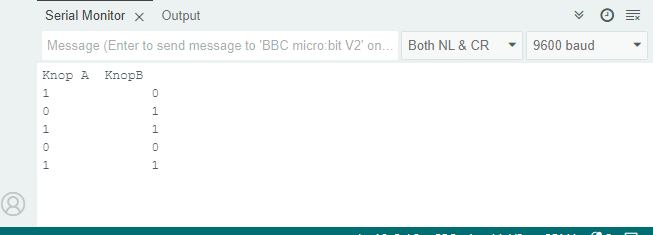
\includegraphics[width=0.6 \linewidth]{figuren/monitorButton}
	\centering
	\caption{Weergave de ingelezen waarde van de bnoppen.}
	\label{fig:button}
\end{figure}
\item De arduino omgeving heeft behalve een \texttt{serial Monitor} ook een \texttt{Serial plotter}. Hierin worden de waarden van de variabele geplot.
De arduino omgeving geeft een korte toelichting op het gebruik van de \href{https://docs.arduino.cc/software/ide-v2/tutorials/ide-v2-serial-plotter/}{serial plotter}. In listing \ref{lst:butplot} zijn twee variabele één variabele heeft altijd de waarde 500, de andere heeft een random waarde.
\begin{lstlisting}[caption={Het uitprinten van een vaste- en een radomwaarde.} ,label={lst:butplot}, numbers=none]
	
int random_variable;
int static_variable = 500;

void setup() {
	Serial.begin(9600);
}

void loop() {
	random_variable = random(0, 1000);
	
	Serial.print("Variable_1:");
	Serial.print(random_variable);
	Serial.print(",");
	Serial.print("Variable_2:");
	Serial.println(static_variable);
	delay(100);
}
	
\end{lstlisting}
Indien deze twee variabel laat uitplotten, wordt iets dergelijks als figuur \ref{fig:plotrnd} weergegeven.
\begin{figure}[H]
	\captionsetup{justification=centering}
	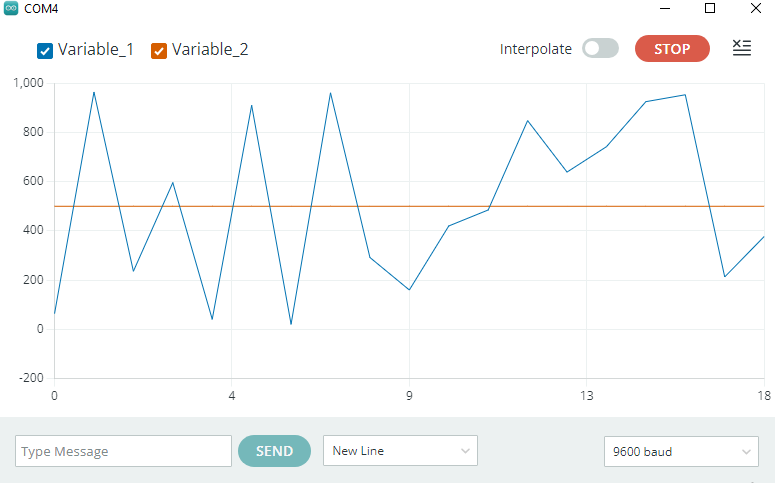
\includegraphics[width=0.7 \linewidth]{figuren/plotVar}
	\centering
	\caption{Het plotten van een vaste en random variabele.}
	\label{fig:plotrnd}
\end{figure}
De \texttt{serial plotter} bepaalt zelf de kleuren van de variabele en de waarde van de Y-as. 
Doordat de waarde van de Y-as bepaald wordt door arduino, kan deze verspringen. Het verspringen van de Y-as kan voorkomen worden door een extra variabele te nemen met een bovengrens, in dit geval is dat 1200.\\
Voeg een bovengrens variabele toe aan listing \ref{lst:butplot} zodat de Y-as gelijk begonnen wordt een maximum van 1200.

\item \label{opd:schakelaar}
Pas de opdracht van \ref{sec:but} \ref{butNr} zodanig aan zodat op de \texttt{Serial plotter} te zien is wanneer een knop is ingedrukt. Zoals weergegeve in figuur \ref{fig:plotBut}.\\ \textbf{TIP}: Bedenk dat \textit{1 + 2 = 3}.
\begin{figure}[H]
	\captionsetup{justification=centering}
	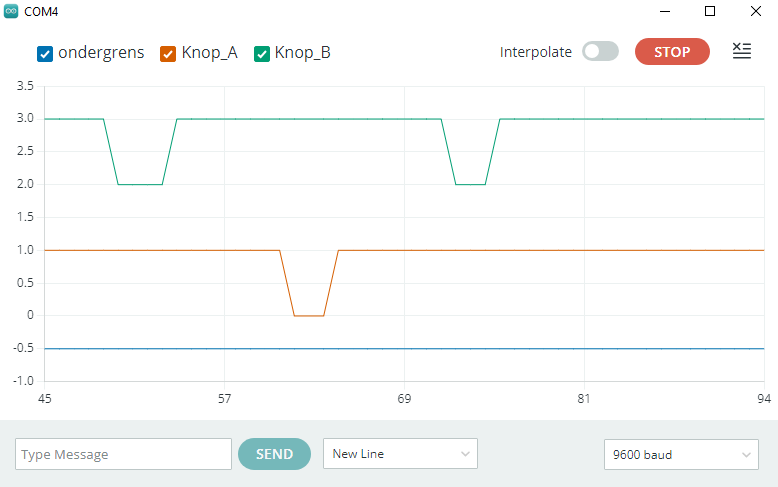
\includegraphics[width=0.8 \linewidth]{figuren/plotBut}
	\centering
	\caption{Het plotten van de stand van de schakelaars met een ondergrens.}
	\label{fig:plotBut}
\end{figure}

\item Op de microbit zit ook een toch sensor zoals in figuur \ref{fig:microbitFront} wordt weergeven en is aangesloten op pin 26. De touch sensor is hierbij zo geconfigureerd dat het eigenlijk een schakelaar is die en 0 of een 1 afgeeft.

Echter het lijkt erop alsof deze niet reageert op het aanraken. Wat helpt is indien je de sensor aanraakt met één van je vingers, met de duim de GND aanraakt, Een andere methode is om je vinger nat te maken, dan wordt oon een 0 afgegeven, zoals te zien is in figuur \ref{fig:plotLog} waar de toch schakelaar de bovenste lijn voorstelt.

\begin{figure}[H]
	\centering

		\begin{subfigure}[b]{0.35\textwidth}
			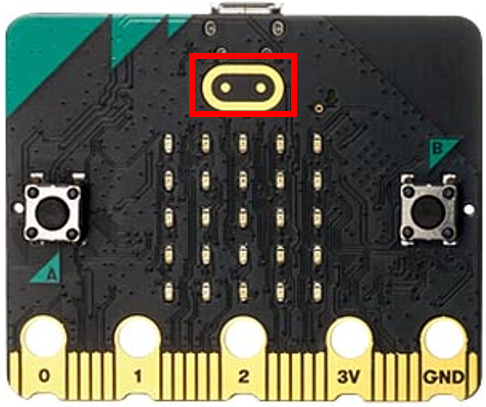
\includegraphics[width=0.95\textwidth]{figuren/microbitFront}
			\caption{Plaats van de touch sensor }
			\label{fig:microbitFront}
		\end{subfigure}
\begin{subfigure}[b]{0.64\textwidth}
	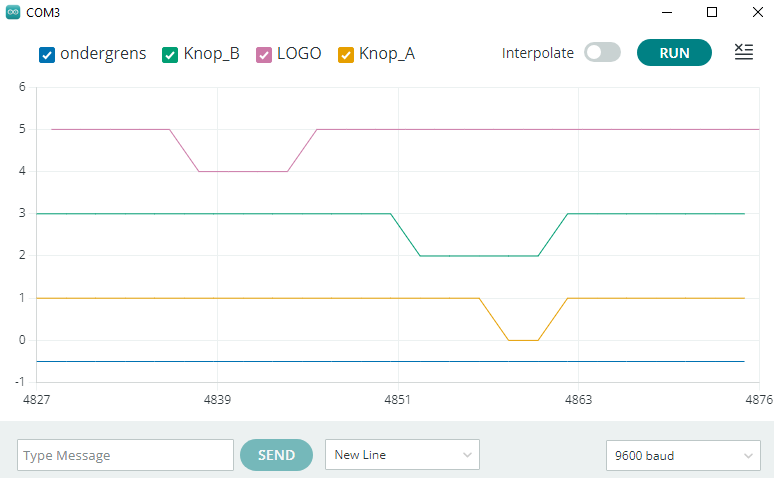
\includegraphics[width=0.95\textwidth]{figuren/plotMetLogo}
	\caption{Het plotten van de inputs }
	\label{fig:plotLog}
	
\end{subfigure}		
		\captionsetup{justification=centering}
	\caption{De touch sensor }
		\label{fig:Logo}

\end{figure}
Breid de opdracht van \ref{opd:schakelaar} uit zodat ook de waarde die de toch schakelaar heeft, wordt weergegeven bij het plotten, zoals te zien is in figuur \ref{fig:plotLog}
\end{enumerate}

\section{Een denderende schakelaar.}

Behalve dat bij het inlezen van de waarde van een externe schakelaar regelmatig een pull\_up weerstand noodzakelijk is. 
Treedt er nog een ander probleem op, namelijk een schakelaar die dendert ook wel bouncing genaamd.

Indien een schakelaar wordt ingedrukt sluit deze bijna nooit in 1 keer, maar veert een aantal keren op en neer. Dit fenomeen wordt weergegeven in Figuur \ref{fig:swDend}, 
\begin{figure}[h!]
	\captionsetup{justification=centering}
	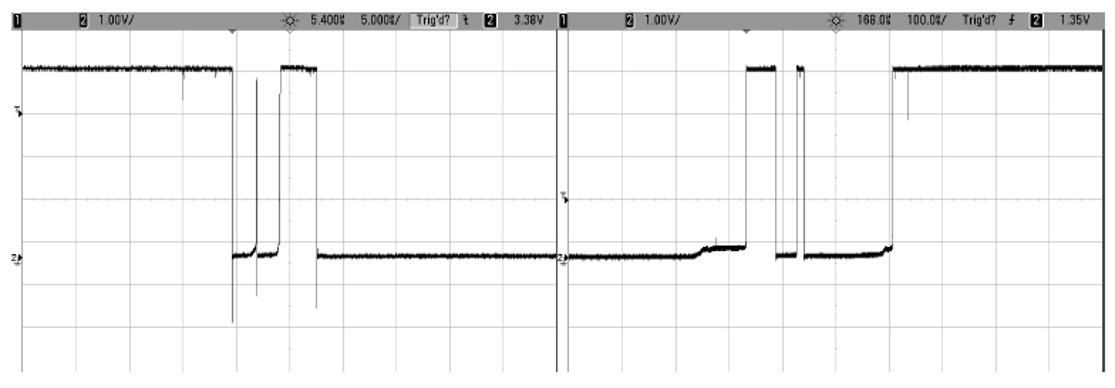
\includegraphics[width=0.6 \linewidth]{figuren/denderen}
	\centering
	\caption{Een denderende schakelaar\cite{williams2014make}.}
	\label{fig:swDend}
\end{figure}
waar te zien is dat bij het indrukken en loslaten van het knopje de schakelaar 'stuitert'. 
Één van de eenvoudigste manieren om dit op te lossen is door even te wachten (een paar milliseconden) en vervolgens te controleren of de knop nog steeds is ingedrukt. Dit wordt weergegeven in listing \ref{lst:denderBut}
%\begin{lstlisting}[style=myArduino, caption= Omgaan met een denderende schakelaar.,label={lst:denderBut}]
%\newpage
\begin{lstlisting}[caption= Omgaan met een denderende schakelaar.,label={lst:denderBut}]
	const int knopA = 5;     // Knop A is aangesloten op poortnummer 5
	const int knopB = 11;    // Knop B is aangesloten op poortnummer 11
	
	void setup() {  
		Serial.begin(9600);
		Serial.println("microbit is ready!");
		
		pinMode(knopA, INPUT);  
		pinMode(knopB, INPUT);   
	}
	boolean isKnopIngedrukt(int); //declaratie van de funcie
	
	void loop(){
		
		if( isKnopIngedrukt(knopA) )
		Serial.println("A is ingedrukt");
		
		if( isKnopIngedrukt(knopB) )
		Serial.println("B is ingedrukt");       
		
		delay(10);
	}
	
	boolean isKnopIngedrukt( int knop) {
		if (! digitalRead(knop)) {  //Is de knop soms ingedrukt ?
			delay(2);      //wacht 2 milliseconde 
			if (! digitalRead(knop)) { //Is knop nog steeds ingedrukt
				return true;
			}
		}
		return false;
	}
\end{lstlisting}

Hierbij wordt in de functie \texttt{\textit{\textcolor{arduinoBlue}{boolean} isKnopIngedrukt(\textcolor{arduinoBlue}{int});}} als eerste gekeken of de knop is ingedrukt, vervolgens wordt er 2 milliseconde gewacht, waarna opnieuw gekeken wordt of de knop is ingedrukt. Is dit zo dan wordt een \textcolor{arduinoBlue}{true} mee teruggegeven anders een \textcolor{arduinoBlue}{false}.

In listing \ref{lst:changeBut} is te zien dat er een detectie plaatsvindt wanneer de toestand van de schakelaar verandert.
\begin{lstlisting}[caption= Een toestandverandering van de schakelaar.,label={lst:changeBut}]
	
	const int COL1 = 4; 
	const int ROW1 = 21;
	const int knopA = 5;     // Knop A is aangesloten op poortnummer 5
	const int knopB = 11;    // Knop B is aangesloten op poortnummer 11
	
	boolean isKnopIngedrukt(int);
	
	int knopTeller = 0;  
	boolean knopToestand = false;
	boolean vorigeKnopToestand = false;
	int ledStatus = LOW;
	
	void setup() {  
		Serial.begin(9600);
		Serial.println("microbit is ready!");
		pinMode(COL1, OUTPUT);
		pinMode(ROW1, OUTPUT);
		pinMode(knopA, INPUT);  
		pinMode(knopB, INPUT);   
		digitalWrite(COL1, LOW);
	}
	
	void loop(){
		knopToestand = isKnopIngedrukt(knopA);
		if(knopToestand != vorigeKnopToestand)  //heeft er een verandering plaatsgevonden?
		if (knopToestand == true) {
			knopTeller++;
			ledStatus = !ledStatus;
			Serial.println(knopTeller);
		}
		delay(50);
		vorigeKnopToestand = knopToestand;
		digitalWrite(ROW1, ledStatus);
	}
	
	boolean isKnopIngedrukt( int knop) {
		if (! digitalRead(knop)) {  //Is de knop soms ingedrukt ?
			delay(2);      //wacht 2 milliseconde 
			if (! digitalRead(knop)) { //Is knop nog steeds ingedrukt
				return true;
			}
		}
		return false;
	}
	
\end{lstlisting}

%Open Bestand $\rightarrow$ Voorbeelden $\rightarrow$ Microbit-HHS $\rightarrow$ 04B.StateChangeDetection en
Download    \href{https://github.com/JohnVi-hhs/embsysP/tree/main/voorbeelden/veranderToestandDrukknop.ino}{voorbeeldcode \ref{lst:changeBut} van GitHub} of kopieer listing \ref{lst:changeBut} en upload het naar de Microbit.
Bestudeer de code en kijk hoe het programma werkt. Het is de bedoeling dat na elke druk op knopA de led aan of uit gaat (wisselt van toestand) en dat de teller steeds met 1 opgehoogd wordt. 
\begin{enumerate}[label=(\Alph*)]
	
	\item In figuur \ref{fig:swToestand} wordt het signaal van de button weergegeven.
	\begin{figure}[h!]
		\captionsetup{justification=centering}
		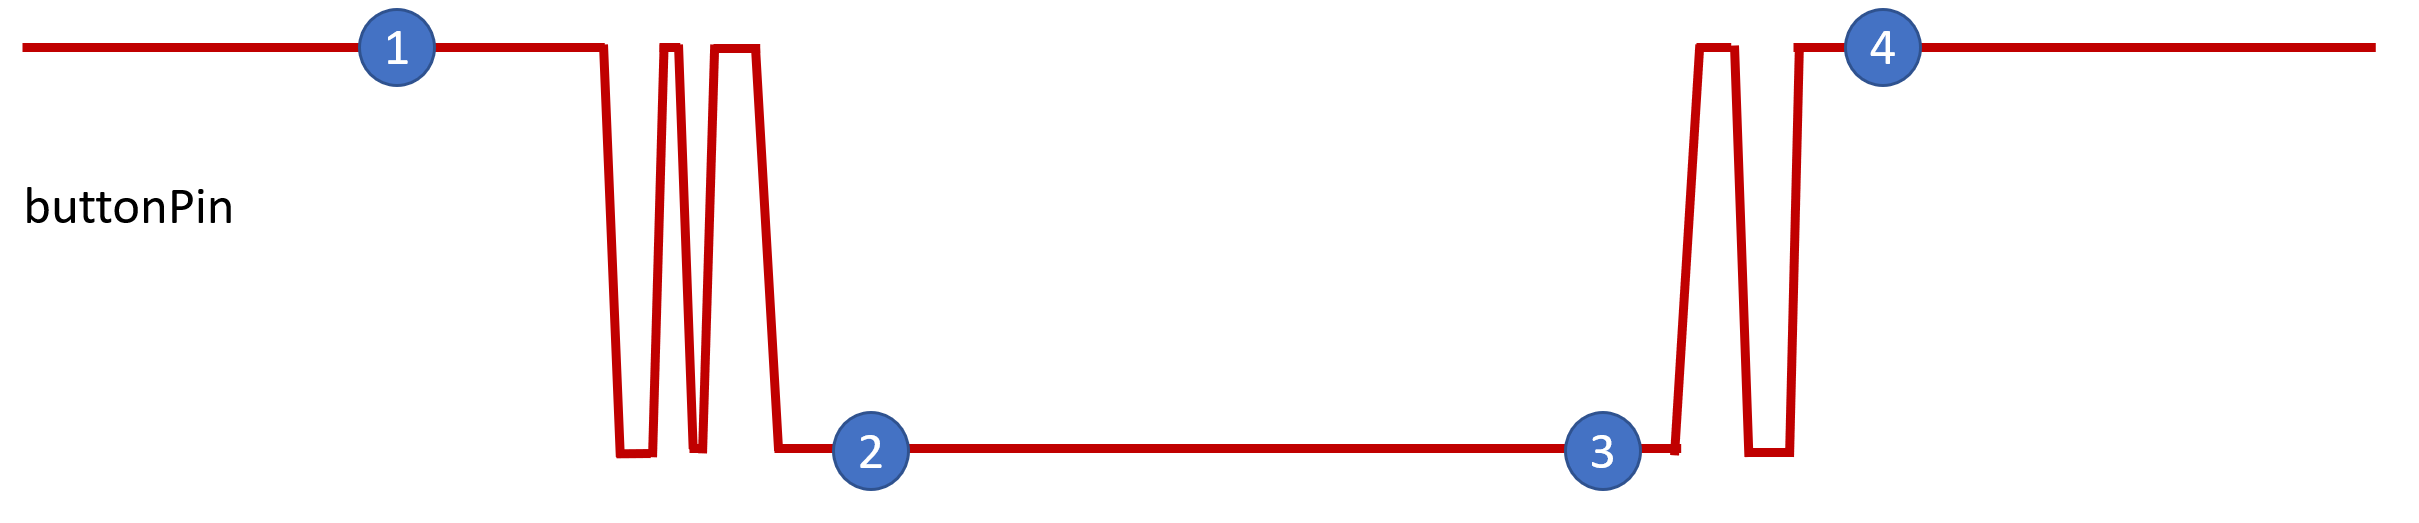
\includegraphics[width=0.8 \linewidth]{figuren/toestandButtonPin}
		\centering
		\caption{Weergaven van het signaal, indien de button wordt ingedrukt en weer wordt losgelaten.}
		\label{fig:swToestand}
	\end{figure}
	In welke toestand (1 t/m 4 )  bevindt zich de variabele \texttt{knopToestand} en \texttt{vorigeKnoptoestand} indien de toestand van de LED verandert en de teller met 1 verhoogd wordt?
	\item Wat is het nut van het statement \textcolor{arduinoOrange}{delay}(50) op regel 31?\hrulefill
	\item Wat is het resultaat indien de outputpin COL1 van listing \ref{lst:changeBut} op \textcolor{arduinoBlue}{HIGH} gezet wordt?	
	\item Breid listing \ref{lst:changeBut} uit, zodat de teller met 1 verlaagd wordt indien met knopB een toestand verandering van 3 naar 4 plaatsvindt.\\
	\textbf{Upload deze opgave op brightspace.}
	
\end{enumerate}

\section{De (externe) pinnen van de microbit}

De Microbit heeft 21 pinnen (aansluitingen) die voor allerlei toepassingen bruikbaar zijn. In figuur \ref{fig:ardPinB} zijn de externe aansluitingen van de microbit te zien. 
\begin{figure}[h!]
	\captionsetup{justification=centering}
	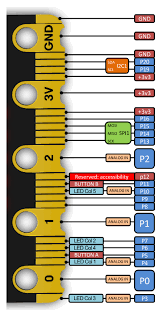
\includegraphics[width=0.4 \linewidth]{figuren/microbitCon}
	\centering
	\caption{Pinlayout van de microbit.}
	\label{fig:ardPinB}
\end{figure}
Hierbij wordt aangegeven welke onderdelen van de microbit ook extern zijn te gebruiken. Bij de pinnen waarbij \fcolorbox{black}{Apricot}{ANALOG IN} staat, kan een externe analoge signaal van b.v. een externe sensor aangesloten worden. De pinnen genaamd \fcolorbox{black}{NavyBlue}{\textcolor{White}{P..}} zijn de pinnummers. In de Arduino IDE kan je die P weglaten en hoef je alleen het nummer op te geven, 0 t/m 20. Uitgebreidere informatie over de pinnen is te vinden op de website \href{https://tech.microbit.org/hardware/edgeconnector/}{tech.microbit.org/hardware/edgeconnector/}.\\
%\newpage

\subsection{Het lezen van externe analoge signalen met de microbit.}

Stel op PIN P0 willen we een externe analoge sensor aansluiten. Voor de spanningswaarde die de sensor levert willen we een digitale waarde weten. 
Dit kan in de Arduino omgeving gedaan worden me het statement:\\

int sensorwaarde = \textcolor{arduinoOrange}{analogRead}(A0);

\begin{enumerate}
	%	\item  Open \textbf{Bestand $\rightarrow$ Voorbeelden $\rightarrow$ 01.Basics $\rightarrow$ AnalogReadSerial}.
	\item In programma listing \ref{lst:analogInp} wordt het analoge signaal van de externe PIN P0 gelezen.
	%\begin{lstlisting}[style=myArduino,numbers=none ,caption= inlezen via een analoog signaal.,label={lst:analogInp}]
	\begin{lstlisting}[numbers=none ,caption= inlezen via een analoog signaal.,label={lst:analogInp}]
	
		void setup() {  
			pinMode(0, INPUT); 
			Serial.begin(9600);
			Serial.println("Hoi embedded programmeurs!");
		}
		
		void loop(){
			// lees de analoge waarde op pin 0:
			int sensorValue = analogRead(A0);
			
			// print de ingelezen analoge waarde
			Serial.println(sensorValue);
			delay(100);        // delay 
		}
		
	\end{lstlisting}
	\begin{enumerate}
		\item  Maak een nieuw Arduino sketch aan en zet listing \ref{lst:analogInp} erin, Klik vervolgens op \img{figuren/ardIcUpl.png} of druk \colorbox{mygray}{\textbf{Ctrl + U}} om het programma te compileren en naar de Microbit te sturen. 
		\item Zoek PIN 0 in Figuur \ref{fig:ardPinB}.
		\item Leg je Microbit op tafel, raak hem niet aan. 
		\item Gebruik de Seriële Plotter om de waarde van de variabele \texttt{\textit{sensorValue}}  te laten zien.
		
		Raak met je vinger het gouden vlakje van pin 0 aan en kijk in de Seriële Plotter wat er gebeurt.
		\item Tussen welke waardes op de linker as liggen de meetwaardes? \hrulefill \\	
		\footnotesize{\texttt{\textit{(Bij mij kwam deze uit tussen de 1000 zonder aanraken en de 750 )}} }
		
	\end{enumerate}
	
	\item De LEDs op de microbit zijn via een truck ook iets wat lichtgevoelig. Hierdoor kan een  bepaalde lichtintentietijd gemeten worden. 
	
	Om deze te kunnen meten zal de LED als een analoge waarde ingelezen moeten worden. 
	In figuur \ref{fig:ledD2} 

	\begin{figure}[h!]
		\centering
		
		\begin{subfigure}[b]{0.30\textwidth}
			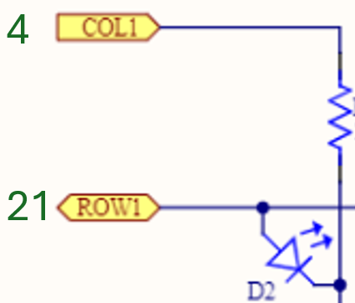
\includegraphics[width=0.95\textwidth]{figuren/ledD2}
			\caption{aansluitschema van LED D2. }
			\label{fig:ledD2}
		\end{subfigure}
		\begin{subfigure}[b]{0.69\textwidth}
			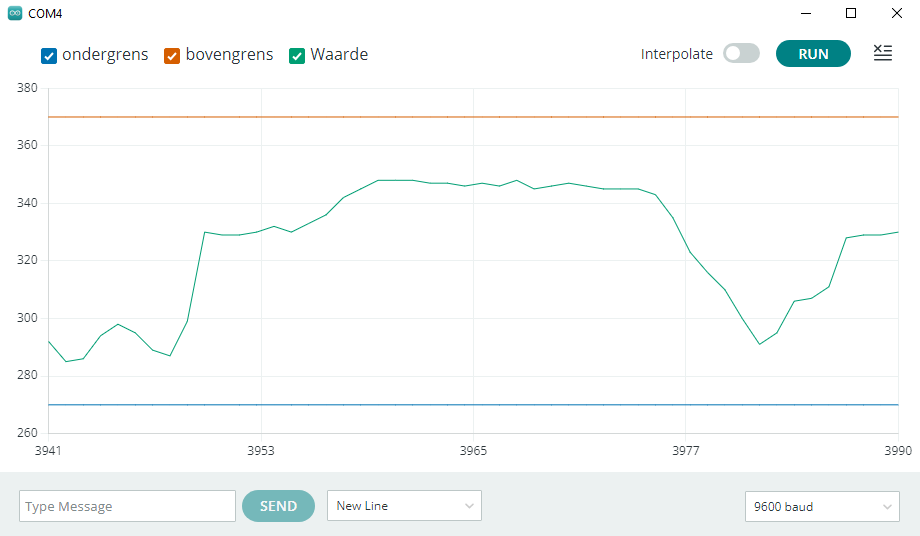
\includegraphics[width=0.97\textwidth]{figuren/plotled}
			\caption{Een idicatie van ontvangen licht. }
			\label{fig:plotLog}
			
		\end{subfigure}		
		\captionsetup{justification=centering}
		\caption{Een matrix LED als fotodiode?  }
		\label{fig:Logo}
	
	\end{figure}
	
	is te zien hoe LED D2 (linkerboven LED van de matrix) is aangesloten. Door nu PIN \textcolor{teal}{4} als een analoge input te definiëren en PIN \textcolor{teal}{21} hoog te maken is er een klein spanningsverschil op PIN 4 te meten.\\
	
    Maak een programma waarbij aan de hand van de middelste LED een indicatie verkregen kan worden over de omgevingslicht.
   
   \subsection{De challenge opdracht}
   
   De micro:bit heeft ook een kompassensor. In listing \ref{lst:kompasInp} wordt de \lstinline|void setup()| en de  \lstinline|void loop()| weergegeven op het kompas uit te lezen. De 
   	\begin{lstlisting}[numbers=none ,caption= De micro:bit als een kompas,label={lst:kompasInp}]
   		
void setup(void) {
	// Start LED matrix driver
	pinMode(ROW3, OUTPUT);
	pinMode(COL3, OUTPUT);
	digitalWrite(COL3, LOW);
	
	// Initialiseer I2C bus.
	DEV_I2C.begin();
	
	Mag.begin();
	Mag.Enable();
	
	Serial.begin(9600);
	pinMode(PIN_BUTTON_A, INPUT);
	// Serial.println("Druk op knopA om te stoppen met kalibreren");
	
	Serial.println("");
	lastDisplayTime = millis();
	kalibreer();
}

   		
void loop(void) {
	float hoek;
	hoek=bepaalHoek();
	if ((millis() - lastDisplayTime) > 1000)  {
		Serial.print("ondergrens:");
		Serial.print(-0.5);
		Serial.print(",");
		Serial.print("Bovengrens:");
		Serial.print(361);
		Serial.print(",");
		Serial.print("Hoek:");
		Serial.println(hoek);
		lastDisplayTime = millis();
	}
	delay(10);
}
   		
   		
\end{lstlisting}
   
   
\end{enumerate}
	

	
	
	\begin{comment}
	
	\item Verander he statement  \textcolor{arduinoOrange}{analogRead}(A0); in \textcolor{arduinoOrange}{digitalRead}(A0); Klik vervolgens op \img{figuren/ardIcUpl.png} of druk \colorbox{mygray}{\textbf{Ctrl + U}} om het programma te compileren en naar de Microbit te sturen. Raak met je vinger het gouden vlakje van pin 0 aan en kijk in de Seriële Plotter wat er gebeurt. 
	
	\item Bij het inlezen van een digitaal signaal is het niet wenselijk dat bij het aanraken van een draadje of een gouden vlakje de ingangswaarde instabiel wordt. Om dit te voorkomen kan bij Arduino de  \textcolor{arduinoBlue}{INPUT\_PULLUP} aangezet worden. Dit wordt gedaan met het statement: \textcolor{arduinoOrange}{pinMode}(0,\textcolor{arduinoBlue}{INPUT\_PULLUP}); 
	
	\begin{minipage}{\linewidth}
		\begin{wrapfigure}[25]{r}{0.54\textwidth}
			\vspace{-15pt}
			\begin{center}
				\centering
				\captionsetup{justification=centering}
				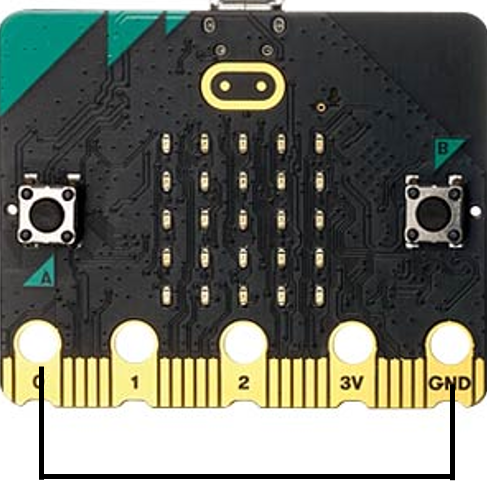
\includegraphics[width=0.32\textwidth]{figuren/microBitDraad}
			\end{center}
			%	\vspace{-14pt}
			\caption{Input verbonden met de GND .}
			\label{fig:micrDraad}
		\end{wrapfigure}
		Zet de \textcolor{arduinoBlue}{INPUT\_PULLUP} aan door het statement 
		\textcolor{arduinoOrange}{pinMode}(0,\textcolor{arduinoBlue}{INPUT\_PULLUP});  
		te plaatsen in de \textcolor{arduinoGreen}{setup} en bekijk wat het resultaat is bij het inlezen van de digitale en analoge waarden. Indien je een draadje bij de hand heb, verbindt de GND met PIN 0, zoals te zien is in figuur \ref{fig:micrDraad}, het gevolg van de PULL\_UP zal zijn dat alleen nog de waarde 0 ingelezen wordt indien de pin ook daadwerkelijk verbonden wordt met de GND.
	\end{minipage}
	
\end{enumerate}

\begin{minipage}{\linewidth}
	\footnotesize{\texttt{\textit{Zoals je ziet is de ingang ongevoelig als je \textcolor{arduinoBlue}{INPUT\_PULLUP} aanzet. Je gebruikt \textcolor{arduinoBlue}{INPUT\_PULLUP} als je een ingang naar een stabiele ‘hoog’ toestand wilt hebben. Je gebruikt deze modus samen met digitalRead() als je een schakelaar wilt uitlezen. Als je de schakelaar indrukt wordt de pin laag.\\
				De knopjes op de Microbit gebruiken een \textbf{externe} pull-up weerstand, met \textcolor{arduinoBlue}{INPUT\_PULLUP} zet je een pull-up weerstand in de microcontroller aan.\\ Kijk eens online voor meer uitleg over de principes van een  \href{https://www.freecodecamp.org/news/a-simple-explanation-of-pull-down-and-pull-up-resistors-660b308f116a/}{pull\_up weerstand}.\\ \\
				Voor verdere uitleg zie \href{https://www.arduino.cc/en/Tutorial/DigitalPins}{www.arduino.cc/en/Tutorial/DigitalPins}
	}}}
\end{minipage}
\normalsize
\end{comment}
\chapter{opdracht 3}

Bij deze opdracht worden LEDs van de bovenste 4 Rijen van de LED matrix van de microkit gedimd.
\begin{enumerate}[label=\Alph*.]
	\item In het onderstaande programma wordt het middelste bit gedimd waarbij de
	$ duty cycle \text{Duty cycle} = \frac{10}{255} \times 100\% = 3.9\%$ is.
	De complete code  is te downloaden als \href{https://github.com/JohnVi-hhs/embsysP/tree/main/voorbeelden/dimOpdracht.ino}{voorbeeldcode \ref{lst:changeBut} van GitHub}
	\begin{lstlisting}[caption= De micro:bit als een kompas,label={lst:dimInp}]
void setup() {  
	
	initMatrix();
	delay(1000);
	analogWrite(ROW3,10);
	
}

void loop(){
}

\end{lstlisting}

\item


	
\end{enumerate}


%\input{deBewegingssensor}
%\input{matrix}
%
\section{Bitwise operaties.}
\label{chap:biw}

Zoals in hoofdstuk \ref{sec:matrix} staat vermeldt heeft de firma Adafruit voor het matrix display een speciale component gemaakt waardoor het matrix display eenvoudig te programmeren is. Listing \ref{lst:matrixaan} is hier een voorbeeld van.
\begin{lstlisting}[caption={Het aanzetten van een LED},label={lst:matrixaan}]
#include <Adafruit_Microbit.h>
#define LED0 0  //definieer LEDx tot een waarde
#define LED1 1
#define LED2 2
#define LED3 3
#define LED4 4

Adafruit_Microbit_Matrix matrixMbit; //maak een LED matrix aan.
const uint8_t
smile_bmp[] =
{ B00000,
	B01010,
	B00000,
	B10001,
	B01110, };
uint8_t matrixje[] =
{ B00000,
	B00000,
	B00000,
	B00000,
	B00000, };

void setup() {
	Serial.begin(9600);
	Serial.println("Welkom bij embedded!");
	
	matrixMbit.begin();
	matrixMbit.show(smile_bmp);
	delay(2000);
	matrixMbit.show(matrixje);
	delay(2000);  
	//zet rechterLED bovenste rij aan
	matrixje[0]= 1 << LED0; //schuif 1, LED0 plaatsen op naar links.
	matrixMbit.show(matrixje);
	delay(2000);  
	//zet linkerLED bovenste rij aan 
	matrixje[0] = 1 << LED4; //schuif 1, LED4 plaatsen op naar links.
	matrixMbit.show(matrixje);
}
void loop() {
}
\end{lstlisting}
Wat opvalt aan Listing \ref{lst:matrixaan} is dat er een hoop define's staan aan het begin. De bedoeling van deze define's is dat de code eenvoudiger te lezen is.
Indien in de code  \small{\texttt{\textit{1 \textless\textless  ~LED4}}} staat, weet de lezer gelijk dat de $4^{e}$ LED bedoeld wordt. Verder is te zien hoe een LED aangezet kan worden door de betreffende bit in een array van 8 bits data, een 1 te maken. Dit wordt gedaan door een 1 (0b00000001) een aantal plaatsen naar links op te laten schuiven. Zoals te zien is in onderstaand statement:\\
\texttt{\textit{matrixje[0]= 1 \textless\textless  ~LED0;}}\\
Hierbij staat de \texttt{1} voor het aantal plaatsen dat LED0 naar links wordt opgeschoven. LED0 staat gedefinieerd op regel 2 van Listing \ref{lst:matrixaan}
\begin{enumerate}
	\item Installeer \href{https://learn.adafruit.com/use-micro-bit-with-arduino/adafruit-libraries}{de Adafruit Libraries} indien dit nog niet gedaan is.
	\item
	\begin{enumerate}

	\item Open voorbeeldcode matrixSmpl (dit is Listing \ref{lst:matrixaan}). 
	\item Breid het programma zodanig zodat uit, zodat zowel LED0 als LED4 van de 2e rij aangaan. Maak hierbij gebruik van de operatoren '\textless\textless' en '\textbar'(bitwise or). Doe dit zoals in de theorie besproken is.
	
%	\begin{table}[h!]
\setlength\arrayrulewidth{2pt}
		\begin{tabular}{|c|c|c|}
			\hline
%			\colorbox{yellow}{\textbf{A}} &\colorbox{yellow}{\textbf{B} & \colorbox{Yellow}{\textbf{AB}}   \\ \hline
          \rowcolor{yellow}
		    A  & B     & A \textbar~ B       \\ \hline          
		    0  & 0     & 0       \\ \hline
			0      & 1     & 1       \\ \hline
			1     & 0     & 1       \\ \hline
			1    & 1     & 1       \\ \hline
		\end{tabular}\\
De bitwise OR 
%	\end{table}
	
	\item Breid het programma uit zodat 2 seconde nadat beide LEDS uit B aangegaan zijn, de linker boven LED (LED4) weer uitgaat. Maak hierbij gebruik van de operatoren '\textless\textless' ,  '\&' en  ' $\sim$'. Doe dit zoals in de theorie besproken is.
	
	\setlength\arrayrulewidth{2pt}
	\begin{tabular}{|c|c|c|}
		\hline
		%			\colorbox{yellow}{\textbf{A}} &\colorbox{yellow}{\textbf{B} & \colorbox{Yellow}{\textbf{AB}}   \\ \hline
		\rowcolor{yellow}
		A  & B     & A \& B       \\ \hline          
		0  & 0     & 0       \\ \hline
		0      & 1     & 0       \\ \hline
		1     & 0     & 0       \\ \hline
		1    & 1     & 1       \\ \hline
	\end{tabular}\\
	De bitwise AND 
	\item Door met bitwise operaties te werken, kan op een eenvoudige wijze een LED dat aan is, uitgezet worden en een LED dat uit is aangezet worden. Dit kan gedaan worden met de exclusief OR operator, zoals te zien is in onderstaand tabel. 
	Breid het programma uit zodat 2 LEDS van de onderste rij aan en uitgaan door de exclusief OR functie te gebruiken. Maak hierbij onder ander gebruik van de operator \^ ~. Do dit zoals in de theorie besproken is.
	
	\setlength\arrayrulewidth{2pt}
	\begin{tabular}{|c|c|c|}
		\hline
		%			\colorbox{yellow}{\textbf{A}} &\colorbox{yellow}{\textbf{B} & \colorbox{Yellow}{\textbf{AB}}   \\ \hline
		\rowcolor{yellow}
		A  & B     & A \^ ~ B       \\ \hline          
		0  & 0     & 0       \\ \hline
		0      & 1     & 1       \\ \hline
		1     & 0     & 1      \\ \hline
		1    & 1     & 0       \\ \hline
	\end{tabular}\\
	De bitwise XOR 
	
	\item Er kan ook getest worden of een LED aan is met behulp van bitwise operatoren.\\	\textcolor{cyan}{uint8\_t} hulpje= matrixje[0];\\
	\textcolor{OliveGreen}{if}(hulpje ...  .....) \{ \\
\}.

Vul het \textcolor{arduinoGreen}{if} statement in en toon aan dat een LED aan of uit is.
 \end{enumerate}

\item In het volgende voorbeeld gaat steeds een LED van rechts naar links aan.

\begin{lstlisting}[caption={Looplicht van de bovenste rij.},label={lst:matrixaan2}]
#include <Adafruit_Microbit.h>

Adafruit_Microbit_Matrix matrixMbit; //maak een LED matrix aan.

uint8_t matrixje[] =
{ B00000,
	B00000,
	B00000,
	B00000,
	B00000, };

void setup() {
	Serial.begin(9600);
	Serial.println("Welkom bij embedded!");

    matrixMbit.begin();
	matrixMbit.show(matrixje);
	delay(1000);  
}

uint8_t nr=0;
uint8_t hulpje;

void loop() {
	hulpje = 1 << nr; //schuif 1, nr plaatsen op naar links.
	matrixje[0]=hulpje; //De bovenste rij van de matrix krijgt de 
	matrixMbit.show(matrixje);
	delay(1000);
	nr++;
	if (nr == 5) {
	    nr=0;
	}        
}
\end{lstlisting}
Op regel 5 wordt een matrix component aangemaakt. Het tonen van de matrix wordt met de show functie gedaan (regel 16 en en 26).

\begin{enumerate}
	\item Download de  \href{https://github.com/JohnVi-hhs/embsysP/tree/main/voorbeelden/matrixloopl.ino}{voorbeeldcode van GitHub} of van brightspace of kopieer listing \ref{lst:matrixaan} in een nieuwe Arduino schets en voer deze uit.\\
	Probeer de uitvoer te verklaren.

\item Maak een functie \texttt{void \textit{zetLedAan}(unint8\_t rij,uint8\_t kolom);} die de LED op kolom en rij aanzet. Maak hierbij gebruik van de bitwise operator \textbar ~ zoals besproken tijdens de les.
\item Maak een functie \texttt{void \textit{zetLedUit}(unint8\_t rij,uint8\_t kolom);} die de LED op kolom en rij uitzet. Maak hierbij gebruik van de bitwise operatoren \& en $\sim$ zoals besproken tijdens de les.
\item Maak een functie \texttt{bool \textit{isLedAan}(unint8\_t rij,uint8\_t kolom);} die checkt of de LED op kolom en rij aan is. Maak hierbij gebruik van een bitmasker zoals besproken tijdens de les.

	\item Pas listing \ref{lst:matrixaan} met behulp van de bovenstaande functies zodanig aan, zodat:
\begin{enumerate}%[label=\arabic*.]
	\item Nadat de eerste rij geweest is, bij de tweede rij de ledjes \'{e}\'{e}n voor \'{e}\'{e}n  aangaan. 
	\item Na de tweede rij bij de derde rij de ledjes \'{e}\'{e}n voor \'{e}\'{e}n  aan gaan. 
	\item Na de laatste rij bij de eerste rij de ledjes \'{e}\'{e}n voor \'{e}\'{e}n  aan gaan. 
\end{enumerate}

\textbf{Upload het resultaat op brightspace.}
\end{enumerate}\label{opdr:loppl}
\item Maak een looplicht dat gaat over alle 5 de rijen van de matrix zoals figuur \ref{fig:loopl} laat zien.

\begin{figure}[H]
	\captionsetup{justification=centering}
\includegraphics[width=0.6 \linewidth]{figuren/looplicht}
\centering
\caption{De volgorde van het looplicht.}
\label{fig:loopl}
\end{figure}

Begin rechtsboven (bit 0 van de ${0^{e}}$ rij in de matrix) en zet vervolgens steeds de LED links aan. Doe dit tot laatste LED van de rij.
Ga 1 rij naar beneden en zet vervolgens de LED rechts van de rij aan. Doe dit tot en met het $1^{e}$ bit.
Ga 1 rij naar beneden en zet vervolgens de LED links van de rij aan. Doe dit tot en met de laatste LED en ga vervolgens een rij naar beneden.
Doe dit tot en met de laatste rij en begin vervolgens weer op de eerste rij, zoals in het volgende filmpje \href{https://www.youtube.com/shorts/8ZyYWEiXsm0} {
	looplicht}
	te zien is.\\
\textbf{Upload het resultaat op brightspace.}
\end{enumerate}

\paragraph{Challenge opdracht}\label{opdr:accSens}

Op de micro:bit zitten verschillende sensoren. Eén van de sensoren is een \href{https://youtu.be/9WAckt2vrrQ}{accelerometer sensor}.
Het programma in listing \ref{lst:acc} toont de x,y en z waarde van de accelerator sensor.
\begin{enumerate}

	\item Download  listing \ref{lst:acc} van \href{https://github.com/JohnVi-hhs/embsysP/tree/main/voorbeelden/accelerator.ino}{ GitHub} of van brightspace of kopieer listing \ref{lst:acc} in een nieuwe arduino omgeving en voer deze uit.
	\item Pas het programma zodanig aan, zodat de LED in de richting beweegt, waarin micro:kit gehouden wordt.

	\end{enumerate}

\begin{lstlisting}[caption={Looplicht van de bovenste rij.},label={lst:acc}]
#include <LSM303AGR_ACC_Sensor.h>

#define DEV_I2C Wire1   // Wire1 is voor de interne I2C bus 
#define LED ROW1 


// Nodig voor de accelerator 
LSM303AGR_ACC_Sensor Acc(&DEV_I2C);


const int COL1 = 4;   
const int ROW1 = 21;   

void setup() {
	// Led.
	
	pinMode(COL1, OUTPUT);
	digitalWrite(COL1, LOW);
	pinMode(ROW1, OUTPUT);
	
	// Initialisatie van de serieele.
	Serial.begin(9600);
	
	// Initialisate I2C bus (wordt veel gebruikt om sensors).
	DEV_I2C.begin();
	
	// Initialisatie van de accelarator.
	Acc.begin();
	Acc.Enable();
	
	uint8_t a;
	Acc.IO_Read(&a,0x0F,1);
	Serial.print("Ik ben: ");
	Serial.println(a);
}

void loop() {
	// Led blinking.
	digitalWrite(LED, HIGH);
	delay(250);
	digitalWrite(LED, LOW);
	delay(250);
	
	// Lees de accelerometer van de LSM303AGR uit.
	int32_t accelerometer[3];
	Acc.GetAxes(accelerometer);
	
	// Output data.
	Serial.print("| Acc[x/y/z] ");
	Serial.print(accelerometer[0]);
	Serial.print(" ");
	Serial.print(accelerometer[1]);
	Serial.print(" ");
	Serial.print(accelerometer[2]);
	Serial.println(" |");
}
\end{lstlisting}




\bibliographystyle{unsrt}
\bibliography{reference}

\input{appendix}
\end{document}
